% Options for packages loaded elsewhere
\PassOptionsToPackage{unicode}{hyperref}
\PassOptionsToPackage{hyphens}{url}
%
\documentclass[
  8pt,
  ignorenonframetext,
]{beamer}
\usepackage{pgfpages}
\setbeamertemplate{caption}[numbered]
\setbeamertemplate{caption label separator}{: }
\setbeamercolor{caption name}{fg=normal text.fg}
\beamertemplatenavigationsymbolsempty
% Prevent slide breaks in the middle of a paragraph
\widowpenalties 1 10000
\raggedbottom
\setbeamertemplate{part page}{
  \centering
  \begin{beamercolorbox}[sep=16pt,center]{part title}
    \usebeamerfont{part title}\insertpart\par
  \end{beamercolorbox}
}
\setbeamertemplate{section page}{
  \centering
  \begin{beamercolorbox}[sep=12pt,center]{part title}
    \usebeamerfont{section title}\insertsection\par
  \end{beamercolorbox}
}
\setbeamertemplate{subsection page}{
  \centering
  \begin{beamercolorbox}[sep=8pt,center]{part title}
    \usebeamerfont{subsection title}\insertsubsection\par
  \end{beamercolorbox}
}
\AtBeginPart{
  \frame{\partpage}
}
\AtBeginSection{
  \ifbibliography
  \else
    \frame{\sectionpage}
  \fi
}
\AtBeginSubsection{
  \frame{\subsectionpage}
}
\usepackage{amsmath,amssymb}
\usepackage{lmodern}
\usepackage{ifxetex,ifluatex}
\ifnum 0\ifxetex 1\fi\ifluatex 1\fi=0 % if pdftex
  \usepackage[T1]{fontenc}
  \usepackage[utf8]{inputenc}
  \usepackage{textcomp} % provide euro and other symbols
\else % if luatex or xetex
  \usepackage{unicode-math}
  \defaultfontfeatures{Scale=MatchLowercase}
  \defaultfontfeatures[\rmfamily]{Ligatures=TeX,Scale=1}
\fi
% Use upquote if available, for straight quotes in verbatim environments
\IfFileExists{upquote.sty}{\usepackage{upquote}}{}
\IfFileExists{microtype.sty}{% use microtype if available
  \usepackage[]{microtype}
  \UseMicrotypeSet[protrusion]{basicmath} % disable protrusion for tt fonts
}{}
\makeatletter
\@ifundefined{KOMAClassName}{% if non-KOMA class
  \IfFileExists{parskip.sty}{%
    \usepackage{parskip}
  }{% else
    \setlength{\parindent}{0pt}
    \setlength{\parskip}{6pt plus 2pt minus 1pt}}
}{% if KOMA class
  \KOMAoptions{parskip=half}}
\makeatother
\usepackage{xcolor}
\IfFileExists{xurl.sty}{\usepackage{xurl}}{} % add URL line breaks if available
\IfFileExists{bookmark.sty}{\usepackage{bookmark}}{\usepackage{hyperref}}
\hypersetup{
  hidelinks,
  pdfcreator={LaTeX via pandoc}}
\urlstyle{same} % disable monospaced font for URLs
\newif\ifbibliography
\usepackage{color}
\usepackage{fancyvrb}
\newcommand{\VerbBar}{|}
\newcommand{\VERB}{\Verb[commandchars=\\\{\}]}
\DefineVerbatimEnvironment{Highlighting}{Verbatim}{commandchars=\\\{\}}
% Add ',fontsize=\small' for more characters per line
\usepackage{framed}
\definecolor{shadecolor}{RGB}{248,248,248}
\newenvironment{Shaded}{\begin{snugshade}}{\end{snugshade}}
\newcommand{\AlertTok}[1]{\textcolor[rgb]{0.94,0.16,0.16}{#1}}
\newcommand{\AnnotationTok}[1]{\textcolor[rgb]{0.56,0.35,0.01}{\textbf{\textit{#1}}}}
\newcommand{\AttributeTok}[1]{\textcolor[rgb]{0.77,0.63,0.00}{#1}}
\newcommand{\BaseNTok}[1]{\textcolor[rgb]{0.00,0.00,0.81}{#1}}
\newcommand{\BuiltInTok}[1]{#1}
\newcommand{\CharTok}[1]{\textcolor[rgb]{0.31,0.60,0.02}{#1}}
\newcommand{\CommentTok}[1]{\textcolor[rgb]{0.56,0.35,0.01}{\textit{#1}}}
\newcommand{\CommentVarTok}[1]{\textcolor[rgb]{0.56,0.35,0.01}{\textbf{\textit{#1}}}}
\newcommand{\ConstantTok}[1]{\textcolor[rgb]{0.00,0.00,0.00}{#1}}
\newcommand{\ControlFlowTok}[1]{\textcolor[rgb]{0.13,0.29,0.53}{\textbf{#1}}}
\newcommand{\DataTypeTok}[1]{\textcolor[rgb]{0.13,0.29,0.53}{#1}}
\newcommand{\DecValTok}[1]{\textcolor[rgb]{0.00,0.00,0.81}{#1}}
\newcommand{\DocumentationTok}[1]{\textcolor[rgb]{0.56,0.35,0.01}{\textbf{\textit{#1}}}}
\newcommand{\ErrorTok}[1]{\textcolor[rgb]{0.64,0.00,0.00}{\textbf{#1}}}
\newcommand{\ExtensionTok}[1]{#1}
\newcommand{\FloatTok}[1]{\textcolor[rgb]{0.00,0.00,0.81}{#1}}
\newcommand{\FunctionTok}[1]{\textcolor[rgb]{0.00,0.00,0.00}{#1}}
\newcommand{\ImportTok}[1]{#1}
\newcommand{\InformationTok}[1]{\textcolor[rgb]{0.56,0.35,0.01}{\textbf{\textit{#1}}}}
\newcommand{\KeywordTok}[1]{\textcolor[rgb]{0.13,0.29,0.53}{\textbf{#1}}}
\newcommand{\NormalTok}[1]{#1}
\newcommand{\OperatorTok}[1]{\textcolor[rgb]{0.81,0.36,0.00}{\textbf{#1}}}
\newcommand{\OtherTok}[1]{\textcolor[rgb]{0.56,0.35,0.01}{#1}}
\newcommand{\PreprocessorTok}[1]{\textcolor[rgb]{0.56,0.35,0.01}{\textit{#1}}}
\newcommand{\RegionMarkerTok}[1]{#1}
\newcommand{\SpecialCharTok}[1]{\textcolor[rgb]{0.00,0.00,0.00}{#1}}
\newcommand{\SpecialStringTok}[1]{\textcolor[rgb]{0.31,0.60,0.02}{#1}}
\newcommand{\StringTok}[1]{\textcolor[rgb]{0.31,0.60,0.02}{#1}}
\newcommand{\VariableTok}[1]{\textcolor[rgb]{0.00,0.00,0.00}{#1}}
\newcommand{\VerbatimStringTok}[1]{\textcolor[rgb]{0.31,0.60,0.02}{#1}}
\newcommand{\WarningTok}[1]{\textcolor[rgb]{0.56,0.35,0.01}{\textbf{\textit{#1}}}}
\usepackage{longtable,booktabs,array}
\usepackage{calc} % for calculating minipage widths
\usepackage{caption}
% Make caption package work with longtable
\makeatletter
\def\fnum@table{\tablename~\thetable}
\makeatother
\setlength{\emergencystretch}{3em} % prevent overfull lines
\providecommand{\tightlist}{%
  \setlength{\itemsep}{0pt}\setlength{\parskip}{0pt}}
\setcounter{secnumdepth}{-\maxdimen} % remove section numbering
% type setting
% ------------------------------------------------------------------------------
\usepackage[german]{babel}     

% fonts
% ------------------------------------------------------------------------------
\usefonttheme{professionalfonts}

% slide title and horizontal line
% ------------------------------------------------------------------------------
\setbeamertemplate{frametitle}{%
    \vskip-30pt \color{black}\large%
    \begin{minipage}[b][23pt]{120mm}%
    \flushleft\insertframetitle%
    \end{minipage}%
}

\setbeamertemplate{headline}										
{
\vskip10pt\hfill\hspace{3.5mm} 										 
\vskip15pt\color{black}\rule{\textwidth}{0.4pt} 					 
}

% slide number
% ---------------------------------------------------------------
\setbeamertemplate{navigation symbols}{}
\setbeamertemplate{footline}
{
\vskip5pt
\vskip2pt
\makebox[123mm]{\hspace{7.5mm}
\hfill Allgemeines Lineares Modell $\vert$ 
\copyright $ $ 2022 Dirk Ostwald CC BY-NC-SA 4.0 $\vert$ 
Folie \insertframenumber}
\vskip4pt
}

% block color scheme
% ------------------------------------------------------------------------------
% colors
\definecolor{white}{RGB}{255,255,255}
\definecolor{grey}{RGB}{235,235,235}
\definecolor{lightgrey}{RGB}{245,245,245}
\definecolor{LightBlue}{RGB}{220,220,255}
\definecolor{darkblue}{RGB}{51, 51, 153}

% definitions and theorems
\setbeamercolor{block title}{fg = black, bg = grey}
\setbeamercolor{block body}{fg = black, bg = lightgrey}

% general line spacing 
% ------------------------------------------------------------------------------
\linespread{1.3}

% local line spacing
% ------------------------------------------------------------------------------
\usepackage{setspace}

% colors
% -----------------------------------------------------------------------------
\usepackage{color}

% justified text
% ------------------------------------------------------------------------------
\usepackage{ragged2e}
\usepackage{etoolbox}
\apptocmd{\frame}{}{\justifying}{}

% bullet point lists
% -----------------------------------------------------------------------------
\setbeamertemplate{itemize item}[circle]
\setbeamertemplate{itemize subitem}[circle]
\setbeamertemplate{itemize subsubitem}[circle]
\setbeamercolor{itemize item}{fg = black}
\setbeamercolor{itemize subitem}{fg = black}
\setbeamercolor{itemize subsubitem}{fg = black}
\setbeamercolor{enumerate item}{fg = black}
\setbeamercolor{enumerate subitem}{fg = black}
\setbeamercolor{enumerate subsubitem}{fg = black}
\setbeamerfont{itemize/enumerate body}{}
\setbeamerfont{itemize/enumerate subbody}{size = \normalsize}
\setbeamerfont{itemize/enumerate subsubbody}{size = \normalsize}

% color links
% ------------------------------------------------------------------------------
\usepackage{hyperref}
\definecolor{urls}{RGB}{204,0,0}
\hypersetup{colorlinks, citecolor = darkblue, urlcolor = urls}


% additional math commands
% ------------------------------------------------------------------------------
\usepackage{bm}                                         
\newcommand{\niton}{\not\owns}
\DeclareMathOperator*{\intinf}{\int_{-\infty}^{\infty}}
\usepackage{mathtools}                                     % pmatrix* environment

% text highlighting
% ------------------------------------------------------------------------------
\usepackage{soul}
\makeatletter
\let\HL\hl
\renewcommand\hl{%
  \let\set@color\beamerorig@set@color
  \let\reset@color\beamerorig@reset@color
  \HL}
\makeatother

% equation highlighting
% -----------------------------------------------------------------------------
\newcommand{\highlight}[2][yellow]{\mathchoice%
  {\colorbox{#1}{$\displaystyle#2$}}%
  {\colorbox{#1}{$\textstyle#2$}}%
  {\colorbox{#1}{$\scriptstyle#2$}}%
  {\colorbox{#1}{$\scriptscriptstyle#2$}}}%

% additional mathematical operators
% ------------------------------------------------------------------------------
\DeclareMathOperator*{\argmax}{arg\,max}
\DeclareMathOperator*{\argmin}{arg\,min}

\ifluatex
  \usepackage{selnolig}  % disable illegal ligatures
\fi
\newlength{\cslhangindent}
\setlength{\cslhangindent}{1.5em}
\newlength{\csllabelwidth}
\setlength{\csllabelwidth}{3em}
\newenvironment{CSLReferences}[2] % #1 hanging-ident, #2 entry spacing
 {% don't indent paragraphs
  \setlength{\parindent}{0pt}
  % turn on hanging indent if param 1 is 1
  \ifodd #1 \everypar{\setlength{\hangindent}{\cslhangindent}}\ignorespaces\fi
  % set entry spacing
  \ifnum #2 > 0
  \setlength{\parskip}{#2\baselineskip}
  \fi
 }%
 {}
\usepackage{calc}
\newcommand{\CSLBlock}[1]{#1\hfill\break}
\newcommand{\CSLLeftMargin}[1]{\parbox[t]{\csllabelwidth}{#1}}
\newcommand{\CSLRightInline}[1]{\parbox[t]{\linewidth - \csllabelwidth}{#1}\break}
\newcommand{\CSLIndent}[1]{\hspace{\cslhangindent}#1}

\author{}
\date{\vspace{-2.5em}}

\begin{document}

\begin{frame}[plain]{}
\protect\hypertarget{section}{}
\center

\begin{center}
\includegraphics[width=0.2\linewidth]{2_Abbildungen/alm_2_otto} \end{center}

\vspace{2mm}

\huge

Allgemeines Lineares Modell \vspace{6mm}

\large

BSc Psychologie SoSe 2022

\vspace{6mm}
\normalsize

Prof.~Dr.~Dirk Ostwald
\end{frame}

\begin{frame}[plain]{}
\protect\hypertarget{section-1}{}
\center
\huge
\vfill

\noindent (2) Korrelation \vfill
\end{frame}

\begin{frame}{}
\protect\hypertarget{section-2}{}
\setstretch{2}
\vfill
\large

Grundlagen

Korrelation und Bestimmtheitsmaß

Korrelation und lineare Abhängigkeit

Korrelation und Regression

Bedingte Korrelation und Partielle Korrelation

Selbstkontrollfragen

\vfill
\end{frame}

\begin{frame}{}
\protect\hypertarget{section-3}{}
\setstretch{2}
\vfill
\large

\textbf{Grundlagen}

Korrelation und Bestimmtheitsmaß

Korrelation und lineare Abhängigkeit

Korrelation und Regression

Bedingte Korrelation und Partielle Korrelation

Selbstkontrollfragen

\vfill
\end{frame}

\begin{frame}{Grundlagen}
\protect\hypertarget{grundlagen}{}
\large

Anwendungsszenario \vspace{2mm}

\begin{center}
\includegraphics[width=0.8\linewidth]{2_Abbildungen/alm_2_beispielszenario} \end{center}
\end{frame}

\begin{frame}{Grundlagen}
\protect\hypertarget{grundlagen-1}{}
Beispieldatensatz

\center
\footnotesize

\(i = 1,...,20\) Patient:innen, \(y_i\) Symptomreduktion bei Patient:in
\(i\), \(x_i\) Anzahl Therapiestunden von Patient:in \(i\)

\setstretch{1}

\begin{longtable}[]{@{}rr@{}}
\toprule
y\_i & x\_i \\
\midrule
\endhead
-3.15 & 1 \\
2.52 & 2 \\
-1.18 & 3 \\
3.06 & 4 \\
1.70 & 5 \\
2.91 & 6 \\
3.92 & 7 \\
2.31 & 8 \\
4.63 & 9 \\
10.91 & 10 \\
17.56 & 11 \\
11.52 & 12 \\
12.31 & 13 \\
12.12 & 14 \\
12.13 & 15 \\
20.37 & 16 \\
25.26 & 17 \\
27.75 & 18 \\
24.93 & 19 \\
32.49 & 20 \\
\bottomrule
\end{longtable}
\end{frame}

\begin{frame}{Grundlagen}
\protect\hypertarget{grundlagen-2}{}
Beispieldatensatz

\begin{center}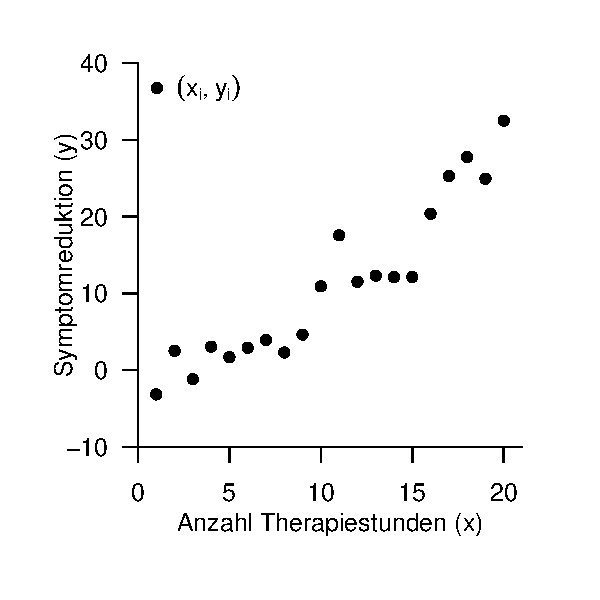
\includegraphics[width=0.55\linewidth]{2_Abbildungen/alm_2_beispieldatensatz} \end{center}

\center

\textcolor{darkblue}{Wie stark hängen Anzahl Therapiestunden und Symptomreduktion zusammen?}
\end{frame}

\begin{frame}{Grundlagen}
\protect\hypertarget{grundlagen-3}{}
\small
\begin{definition}[Korrelation]
\justifying
Die \textit{Korrelation} zweier Zufallsvariablen $X$ und $Y$ ist definiert als
\begin{equation}
\rho(X,Y) := \frac{\mathbb{C}(X,Y)}{\mathbb{S}(X)\mathbb{S}(Y)}
\end{equation}
wobei $\mathbb{C}(X,Y)$ die Kovarianz von $X$ und $Y$ und $\mathbb{V}(X)$ und
$\mathbb{V}(Y)$ die Varianzen von $X$ und $Y$, respektive, bezeichnen.
\end{definition}

\footnotesize

Bemerkungen

\begin{itemize}
\tightlist
\item
  \(\rho(X,Y)\) wird auch \textit{Korrelationskoeffizient} von \(X\) und
  \(Y\) genannt.
\item
  Wir haben bereits gesehen, dass \(-1 \le \rho(X,Y) \le 1\) gilt.
\item
  Wenn \(\rho(X,Y) = 0\) ist, werden \(X\) und \(Y\)
  \textit{unkorreliert} genannt.
\item
  Wir haben bereits gesehen, dass aus der Unabhängigkeit von \(X\) und
  \(Y\), folgt dass \(\rho(X,Y) = 0\).
\item
  Aus \(\rho(X,Y) = 0\) folgt aber wie bereits gesehen die
  Unabhängigkeit von \(X\) und \(Y\) im Allgemeinen nicht.
\end{itemize}
\end{frame}

\begin{frame}{Grundlagen}
\protect\hypertarget{grundlagen-4}{}
\footnotesize
\begin{definition}[Stichprobenkorrelation]
\justifying
$\{(x,y_1),...,(x_n,y_n)\} \subset \mathbb{R}$ sei eine Wertemenge. Weiterhin seien:
\begin{itemize}
\item Die Stichprobenmittel der $x_i$ und $y_i$ definiert als
\begin{equation}
\bar{x} := \frac{1}{n}\sum_{i=1}^n x_i
\mbox{ und }
\bar{y} := \frac{1}{n}\sum_{i=1}^n y_i.
\end{equation}
\item Die Stichprobenstandardabweichungen $x_i$ und $y_i$ definiert als
\begin{equation}
s_x := \sqrt{\frac{1}{n-1}(x_i - \bar{x})^2}
\mbox{ und }
s_y := \sqrt{\frac{1}{n-1}(y_i - \bar{y})^2}.
\end{equation}
\item Die Stichprobenkovarianz der $(x,y_1),...,(x_n,y_n)$ definiert als
\begin{equation}
c_{xy} := \frac{1}{n-1}\sum_{i=1}^n (x_i - \bar{x}_n)(y_i - \bar{y}_n).
\end{equation}
\end{itemize}
Dann ist die \textit{Stichprobenkorrelation} der $(x,y_1),...,(x_n,y_n)$ definiert als
\begin{equation}
r_{xy} := \frac{c_{xy}}{s_xs_y}
\end{equation}
und  wird auch \textit{Stichprobenkorrelationskoeffizient} genannt.
\end{definition}
\end{frame}

\begin{frame}[fragile]{Grundlagen}
\protect\hypertarget{grundlagen-5}{}
Beispiel \vspace{2mm} \tiny \setstretch{1.2}

\begin{Shaded}
\begin{Highlighting}[]
\CommentTok{\# Laden des Beispieldatensatzes}
\NormalTok{fname }\OtherTok{=} \FunctionTok{file.path}\NormalTok{(}\FunctionTok{getwd}\NormalTok{(), }\StringTok{"2\_Daten"}\NormalTok{, }\StringTok{"2\_Korrelation\_Beispieldatensatz.csv"}\NormalTok{)     }\CommentTok{\# Dateipfad}
\NormalTok{D     }\OtherTok{=} \FunctionTok{read.table}\NormalTok{(fname, }\AttributeTok{sep =} \StringTok{","}\NormalTok{, }\AttributeTok{header =} \ConstantTok{TRUE}\NormalTok{)                              }\CommentTok{\# Laden als Dataframe}
\NormalTok{x\_i   }\OtherTok{=}\NormalTok{ D}\SpecialCharTok{$}\NormalTok{x\_i                                                                    }\CommentTok{\# x\_i Werte}
\NormalTok{y\_i   }\OtherTok{=}\NormalTok{ D}\SpecialCharTok{$}\NormalTok{y\_i                                                                    }\CommentTok{\# y\_i Werte}
\NormalTok{n     }\OtherTok{=} \FunctionTok{length}\NormalTok{(x\_i)                                                              }\CommentTok{\# n}

\CommentTok{\# "Manuelle" Berechnung der Stichprobenkorrelation}
\NormalTok{x\_bar }\OtherTok{=}\NormalTok{ (}\DecValTok{1}\SpecialCharTok{/}\NormalTok{n)}\SpecialCharTok{*}\FunctionTok{sum}\NormalTok{(x\_i)                                                           }\CommentTok{\# \textbackslash{}bar\{x\}}
\NormalTok{y\_bar }\OtherTok{=}\NormalTok{ (}\DecValTok{1}\SpecialCharTok{/}\NormalTok{n)}\SpecialCharTok{*}\FunctionTok{sum}\NormalTok{(y\_i)                                                           }\CommentTok{\# \textbackslash{}bar\{y\}}
\NormalTok{s\_x   }\OtherTok{=} \FunctionTok{sqrt}\NormalTok{(}\DecValTok{1}\SpecialCharTok{/}\NormalTok{(n}\DecValTok{{-}1}\NormalTok{)}\SpecialCharTok{*}\FunctionTok{sum}\NormalTok{((x\_i }\SpecialCharTok{{-}}\NormalTok{ x\_bar)}\SpecialCharTok{\^{}}\DecValTok{2}\NormalTok{))                                       }\CommentTok{\# s\_x}
\NormalTok{s\_y   }\OtherTok{=} \FunctionTok{sqrt}\NormalTok{(}\DecValTok{1}\SpecialCharTok{/}\NormalTok{(n}\DecValTok{{-}1}\NormalTok{)}\SpecialCharTok{*}\FunctionTok{sum}\NormalTok{((y\_i }\SpecialCharTok{{-}}\NormalTok{ y\_bar)}\SpecialCharTok{\^{}}\DecValTok{2}\NormalTok{))                                       }\CommentTok{\# s\_y}
\NormalTok{c\_xy  }\OtherTok{=} \DecValTok{1}\SpecialCharTok{/}\NormalTok{(n}\DecValTok{{-}1}\NormalTok{) }\SpecialCharTok{*} \FunctionTok{sum}\NormalTok{((x\_i }\SpecialCharTok{{-}}\NormalTok{ x\_bar) }\SpecialCharTok{*}\NormalTok{ (y\_i }\SpecialCharTok{{-}}\NormalTok{ y\_bar))                             }\CommentTok{\# c\_\{xy\}}
\NormalTok{r\_xy  }\OtherTok{=}\NormalTok{ c\_xy}\SpecialCharTok{/}\NormalTok{(s\_x }\SpecialCharTok{*}\NormalTok{ s\_y)                                                         }\CommentTok{\# r\_\{xy\}}
\FunctionTok{print}\NormalTok{(r\_xy)                                                                      }\CommentTok{\# Ausgabe}
\end{Highlighting}
\end{Shaded}

\begin{verbatim}
> [1] 0.938
\end{verbatim}

\begin{Shaded}
\begin{Highlighting}[]
\CommentTok{\# Automatische Berechnung mit cor()}
\NormalTok{r\_xy  }\OtherTok{=} \FunctionTok{cor}\NormalTok{(x\_i,y\_i)                                                             }\CommentTok{\# r\_\{xy\}}
\FunctionTok{print}\NormalTok{(r\_xy)                                                                      }\CommentTok{\# Ausgabe}
\end{Highlighting}
\end{Shaded}

\begin{verbatim}
> [1] 0.938
\end{verbatim}

\center

\(\Rightarrow\) Anzahl Therapiestunden und Symptomreduktion sind
hochkorreliert.
\end{frame}

\begin{frame}{Grundlagen}
\protect\hypertarget{grundlagen-6}{}
Mechanik der Kovariationsterme

\begin{center}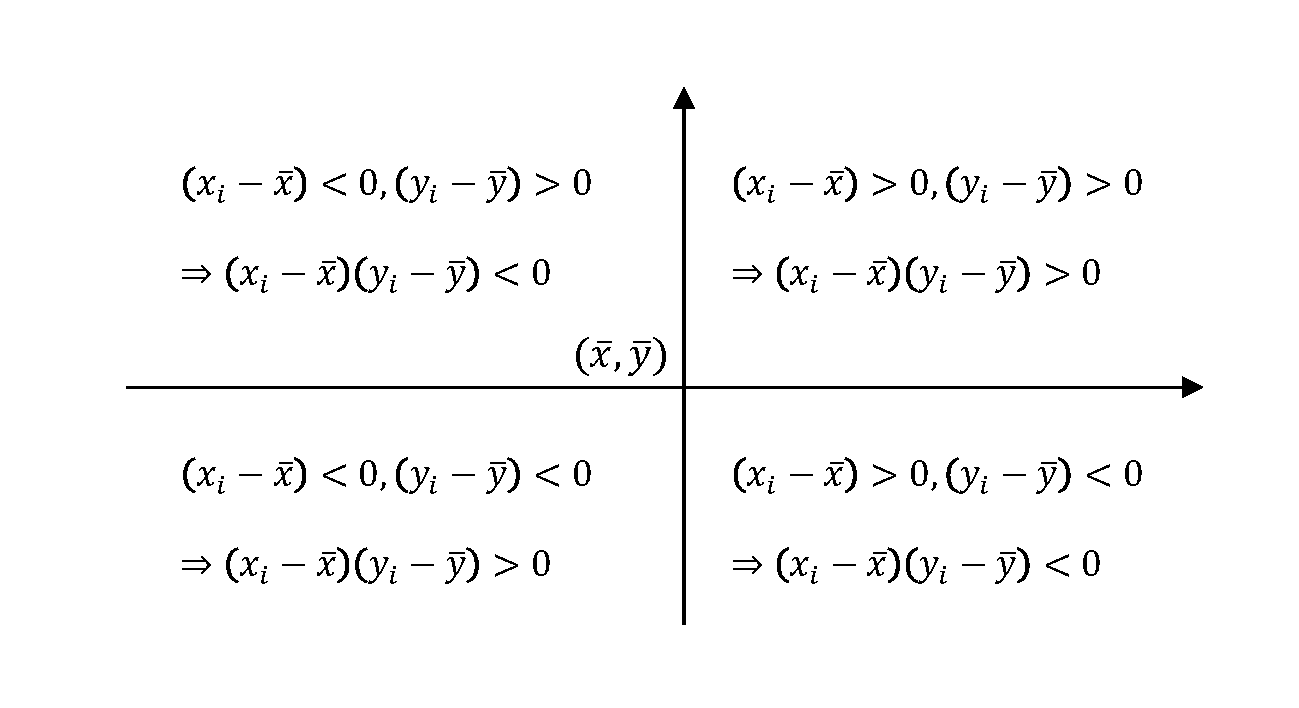
\includegraphics[width=0.8\linewidth]{2_Abbildungen/alm_2_korrelationsterme} \end{center}

\center
\footnotesize

Häufige richtungsgleiche Abweichung der \(x_i\) und \(y_i\) von ihren
Mittelwerten \(\Rightarrow\) Positive Korrelation

Häufige richtungsungleiche Abweichung der \(x_i\) und \(y_i\) von ihren
Mittelwerten \(\Rightarrow\) Negative Korrelation

Keine häufigen richtungsgleichen oder -entgegengesetzten Abweichungen
\(\Rightarrow\) Keine Korrelation
\end{frame}

\begin{frame}{Grundlagen}
\protect\hypertarget{grundlagen-7}{}
\vspace{2mm}

Beispiele

\begin{center}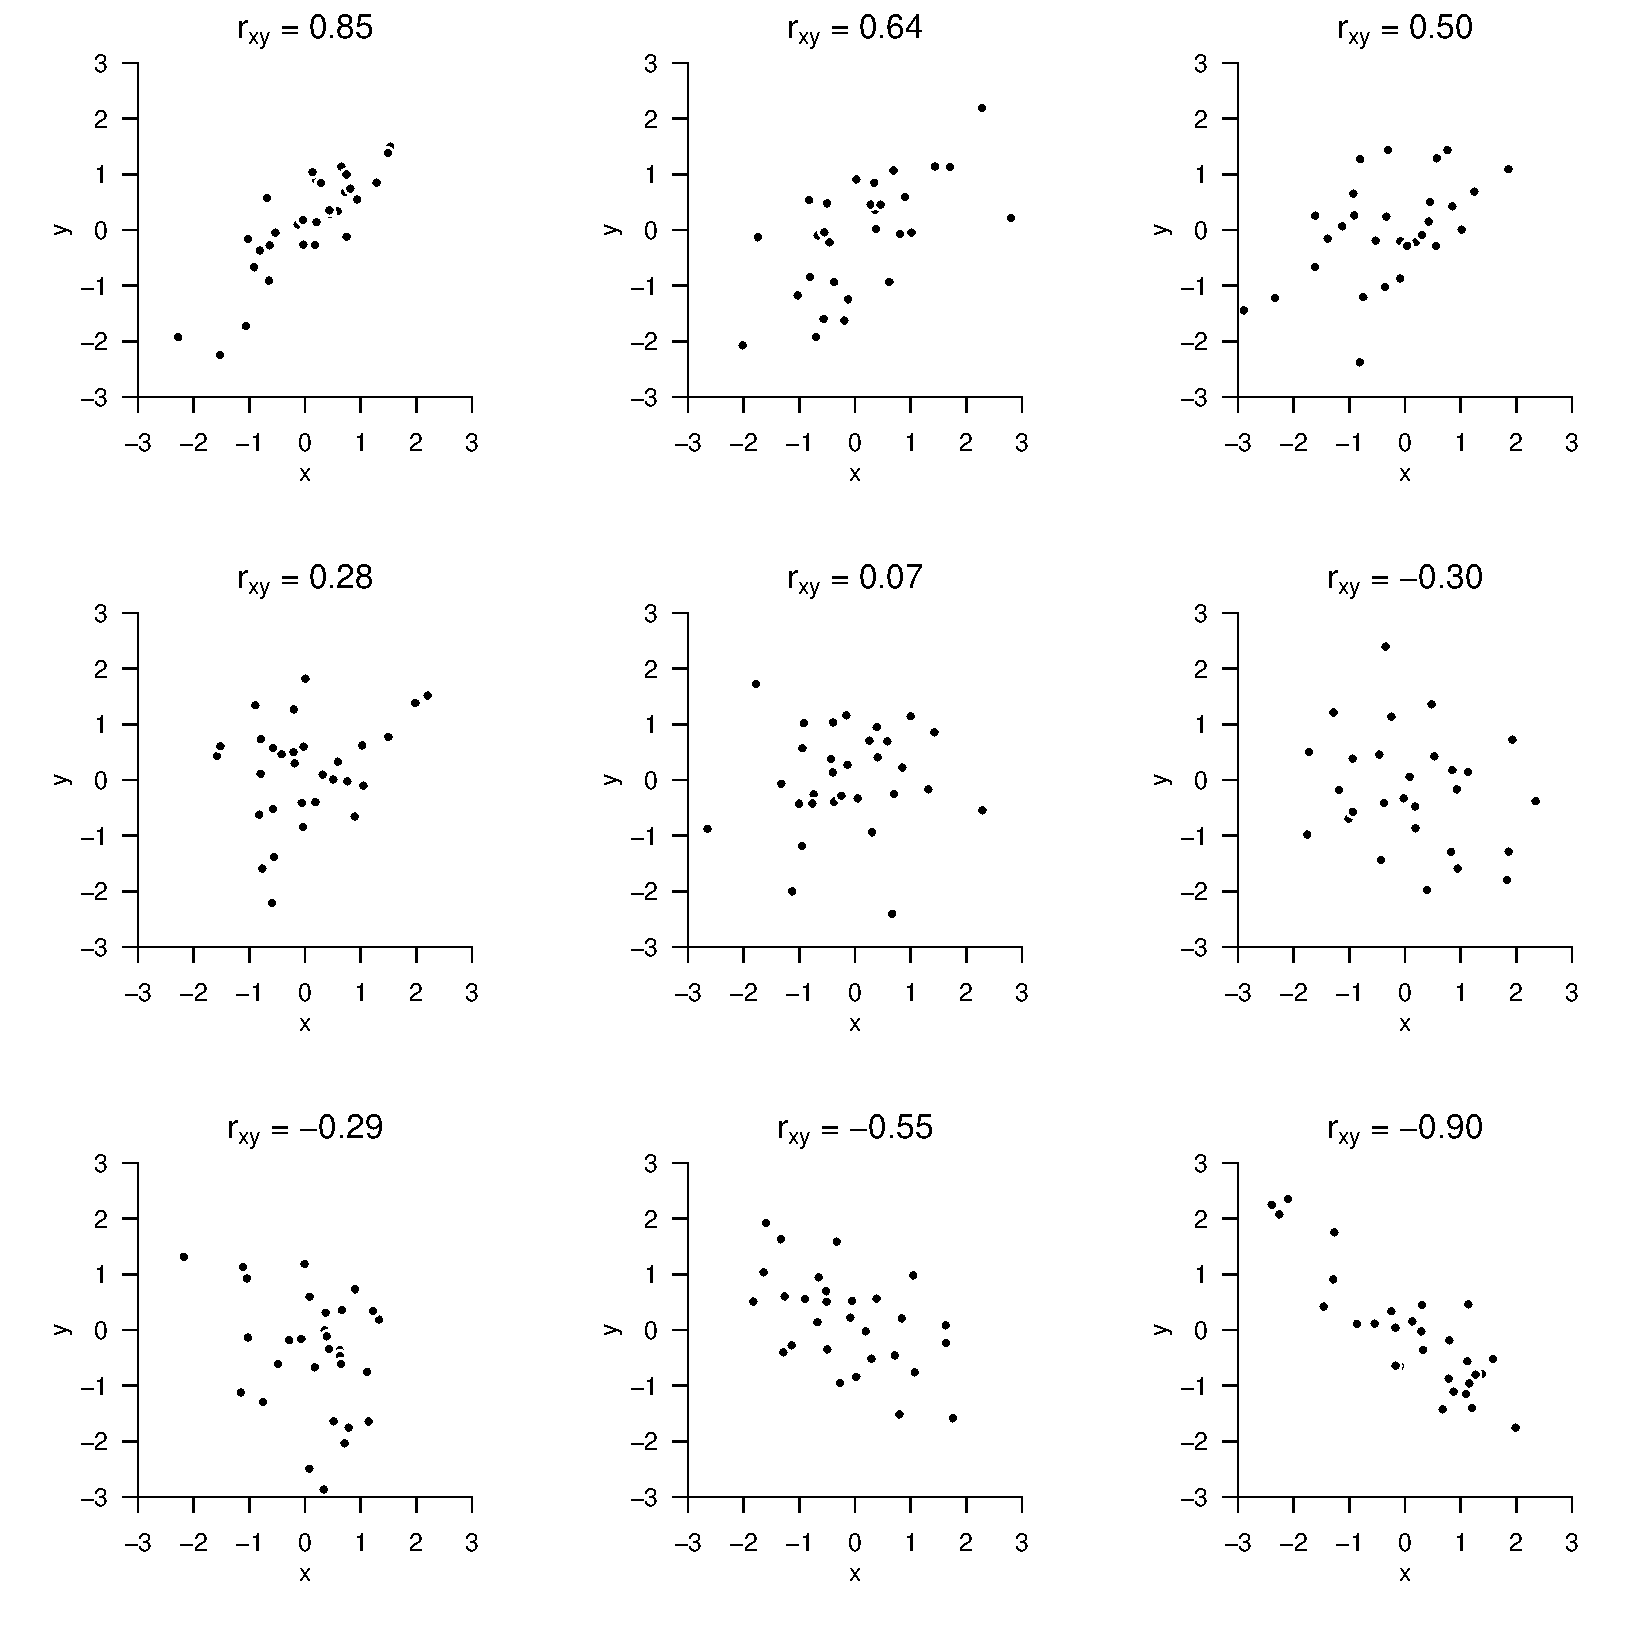
\includegraphics[width=0.6\linewidth]{2_Abbildungen/alm_2_korrelationsbeispiele} \end{center}
\end{frame}

\begin{frame}{Grundlagen}
\protect\hypertarget{grundlagen-8}{}
\footnotesize
\begin{theorem}[Stichprobenkorrelation bei linear-affinen Transformationen]
\justifying
\normalfont
Für eine Wertemenge $\{(x_i,y_i)\}_{i = 1,...n} \subset \mathbb{R}^2$ sei
$\{(\tilde{x}_i,\tilde{y}_i)\}_{i = 1,...n} \subset \mathbb{R}^2$ eine linear-affin
transformierte Wertemenge mit
\begin{equation}
(\tilde{x}_i, \tilde{y}_i) = (a_x x_i + b_x, a_y y_i + b_y), a_x,a_y \neq 0.
\end{equation}
Dann gilt
\begin{equation}
|r_{\tilde{x}\tilde{y}}| = |r_{xy}|.
\end{equation}
\end{theorem}

Bemerkungen

\begin{itemize}
\tightlist
\item
  Der Betrag der Stichprobenkorrelation ändert sich bei linear-affiner
  Datentransformation nicht.
\item
  Man sagt, dass die Stichprobenkorrelation im Gegensatz zur
  Stichprobenkovarianz \textit{maßstabsunabhängig} ist.
\end{itemize}
\end{frame}

\begin{frame}{Grundlagen}
\protect\hypertarget{grundlagen-9}{}
\footnotesize
\vspace{1mm}

\underline{Beweis}

Es gilt \tiny \begin{align}
\begin{split}
r_{\tilde{x}\tilde{y}}
& := \frac{\frac{1}{n-1}\sum_{i=1}^n (\tilde{x}_i - \bar{\tilde{x}})(\tilde{y}_i - \bar{\tilde{y}})}
        {\sqrt{\frac{1}{n-1}(\sum_{i=1}^n\tilde{x}_i - \bar{\tilde{x}})^2} \sqrt{\frac{1}{n-1}(\sum_{i=1}^n\tilde{y}_i - \bar{\tilde{y}})^2}}
\\
&  = \frac{\sum_{i=1}^n (a_x x_i + b_x - (a_x\bar{x} + b_x))(a_y y_i + b_y - (a_y \bar{y} + b_y))}
          {\sqrt{\sum_{i=1}^n (a_x x_i + b_x - (a_x \bar{x} + b_x))^2}\sqrt{\sum_{i=1}^n (a_y y_i + b_y - (a_y \bar{y} + b_y))^2}}
\\
&  = \frac{a_x a_y\sum_{i=1}^n (x_i-\bar{x})(y_i-\bar{y})}
          {\sqrt{a_x^2\sum_{i=1}^n (x_i  - \bar{x})^2}\sqrt{a_y^2\sum_{i=1}^n (y_i - \bar{y})^2}}
\\
&  = \frac{a_x a_y}{|a_x||a_y|}
     \frac{\sum_{i=1}^n (x_i-\bar{x})(y_i-\bar{y})}
          {\sqrt{\sum_{i=1}^n (x_i  - \bar{x})^2}\sqrt{\sum_{i=1}^n (y_i - \bar{y})^2}}
\\
&  = \frac{a_x a_y}{|a_x||a_y|}\frac{c_{xy}}{s_x s_y}
\\
&  = \frac{a_x a_y}{|a_x||a_y|}r_{xy}.
\end{split}
\end{align} \footnotesize Also folgt, durch Durchspielen aller möglichen
Vorzeichenfälle, dass \begin{equation}
|r_{\tilde{x}\tilde{y}}| = |r_{xy}|.
\end{equation} \(\hfill\Box\)
\end{frame}

\begin{frame}{}
\protect\hypertarget{section-4}{}
\setstretch{2}
\vfill
\large

Grundlagen

\textbf{Korrelation und Bestimmtheitsmaß}

Korrelation und lineare Abhängigkeit

Korrelation und Regression

Bedingte Korrelation und Partielle Korrelation

Selbstkontrollfragen

\vfill
\end{frame}

\begin{frame}{Korrelation und Bestimmtheitsmaß}
\protect\hypertarget{korrelation-und-bestimmtheitsmauxdf}{}
Überblick \setstretch{2} \footnotesize

Das sogenannte Bestimmtheitsmaß \(\mbox{R}^2\) ist eine beliebte
Statistik.

Numerisch ist \(\mbox{R}^2\) das Quadrat des
Stichprobenkorrelationskoeffizienten.

Ist die Stichprobenkorrelation \(r_{xy} = 0.5\), dann ist
\(\mbox{R}^2 = 0.25\), ist \(r_{xy} = -0.5\), dann ist
\(\mbox{R}^2 = 0.25\).

\(\Rightarrow \mbox{R}^2\) enthält also weniger Information über die
Rohdaten als \(r_{xy}\), da das Vorzeichen wegfällt.

\(\Rightarrow\) \textit{Perse} ist die Angabe von \(\mbox{R}^2\)
anstelle von \(r_{xy}\) im Kontext der Korrelation zweier Variablen
wenig sinnvoll.

Ein tieferes Verständnis von \(\mbox{R}^2\) erlaubt jedoch

\begin{enumerate}
[(1)]
\tightlist
\item
  Einen Einstieg in das Konzept von Quadratsummenzerlegungen, einem
  wichtigen ALM Evaluationsprinzip.
\item
  Einen Einstieg in das Verständnis der Zusammenhänge von
  Ausgleichsgerade und Stichprobenkorrelation.
\item
  Einen ersten Einblick in die Tatsache, dass Korrelationen (nur)
  linear-affine Zusammenhänge quantifizieren.
\end{enumerate}
\end{frame}

\begin{frame}{Korrelation und Bestimmtheitsmaß}
\protect\hypertarget{korrelation-und-bestimmtheitsmauxdf-1}{}
\small
\begin{definition}[Erklärte Werte und Residuen einer Ausgleichsgerade]
\justifying
Gegeben seien eine Wertemenge $\{(x,y_1), ..., (x_n,y_n)\} \subset \mathbb{R}^2$
und die zu dieser Wertemenge gehörende Ausgleichsgerade
\begin{equation}
f_{\hat{\beta}} : \mathbb{R} \to \mathbb{R}, x \mapsto f_{\hat{\beta}}(x) := \hat{\beta}_0 + \hat{\beta}_1x
\end{equation}
Dann werden für $i = 1,...,n$
\begin{equation}
\hat{y}_i := \hat{\beta}_0 + \hat{\beta}_1x_i
\end{equation}
die durch die Ausgleichsgerade \textit{erklärten Werte} genannt und
\begin{equation}
\hat{\varepsilon}_i := y_i - \hat{y}_i
\end{equation}
die \textit{Residuen} der Ausgleichsgerade genannt.
\end{definition}
\end{frame}

\begin{frame}{Korrelation und Bestimmtheitsmaß}
\protect\hypertarget{korrelation-und-bestimmtheitsmauxdf-2}{}
Erklärte Werte und Residuen

\begin{center}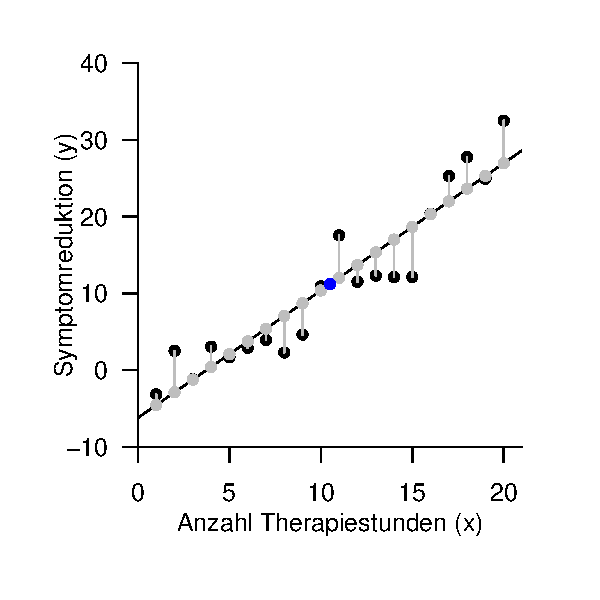
\includegraphics[width=0.55\linewidth]{2_Abbildungen/alm_2_erklaertewerte_residuen} \end{center}

\vspace{-5mm}
\center

\(\bullet \, (x_i, y_i)\) \hspace{2mm} \textcolor{blue}{$\bullet$}
\((\bar{x},\bar{y})\) \hspace{2mm} \textbf{---} \(f_{\hat{\beta}}(x)\)
\hspace{2mm} \textcolor{lightgray}{$\bullet$} \(\hat{y}_i\) \hspace{2mm}
\textcolor{lightgray}{\textbf{---}} \(\hat{\varepsilon}_i\) \hspace{2mm}
\(i = 1,...,n\)
\end{frame}

\begin{frame}{Korrelation und Bestimmtheitsmaß}
\protect\hypertarget{korrelation-und-bestimmtheitsmauxdf-3}{}
\small
\begin{theorem}[Quadratsummenzerlegung bei Ausgleichsgerade]
\justifying
\normalfont
Für eine Wertemenge $\{(x,y_1), ..., (x_n,y_n)\} \subset \mathbb{R}^2$ und ihre
zugehörige Ausgleichsgerade $f_{\hat{\beta}}$ seien für
\begin{equation}
\bar{y} := \frac{1}{n}\sum_{i=1}^n y_i \mbox{ und }
\hat{y}_i := \hat{\beta}_0 + \hat{\beta}_1x_i, \mbox{ für } i= 1,...,n
\end{equation}
das Stichprobenmittel der $y$-Werte und die durch die Ausgleichsgerade erklärten Werte,
respektive. Weiterhin seien

\center
\vspace{1mm}
\begin{tabular}{ll}
$\mbox{SQT} := \sum_{i = 1}^n (y_i - \bar{y})^2$          & die \textit{Total Sum of Squares}      \\\\
$\mbox{SQE} := \sum_{i = 1}^n (\hat{y}_i - \bar{y})^2$    & die \textit{Explained Sum of Squares}  \\\\
$\mbox{SQR} := \sum_{i = 1}^n (y_i - \hat{y}_i)^2$        & die \textit{Residual Sum of Squares}   \\
\end{tabular}
\vspace{1mm}
\flushleft
Dann gilt
\begin{equation}
\mbox{SQT} = \mbox{SQE} + \mbox{SQR}
\end{equation}
\end{theorem}
\end{frame}

\begin{frame}{Korrelation und Bestimmtheitsmaß}
\protect\hypertarget{korrelation-und-bestimmtheitsmauxdf-4}{}
\footnotesize
\setstretch{1.4}

Bemerkungen

\begin{itemize}
\item SQT repräsentiert die Gesamtstreung der $y_i$-Werte um ihren Mittelwert $\bar{y}$.
\item SQE repräsentiert die Streuung der erklärten Werte $\hat{y}_i$ um ihren Mittelwert
\item[] $\Rightarrow$ Große Werte von SQE repräsentieren eine große absolute Steigung der $y_i$ mit den $x_i$
\item[] $\Rightarrow$ Kleine Werte von SQE repräsentieren eine kleine absolute Steigung der $y_i$ mit den $x_i$
\item SQE ist also ein Maß für die Stärke des linearen Zusammenhangs der $x$- und $y$-Werte
\item SQR ist die Summe der quadrierten Residuen, es gilt
\begin{equation}
\mbox{SQR} := \sum_{i = 1}^n (y_i - \hat{y}_i)^2 := \sum_{i=1}^n \hat{\varepsilon}_i^2
\end{equation}
\item[] $\Rightarrow$ Große Werte von SQR repräsentieren große Abweichungen der erklärten von den beobachteten $y$-Werten
\item[] $\Rightarrow$ Kleine Werte von SQR repräsentieren geringe Abweichungen der erklärten von den beobachteten $y$-Werten
\item SQR ist also ein Maß für die Güte der Beschreibung der Datenmenge durch die Ausgleichsgerade.
\end{itemize}
\end{frame}

\begin{frame}{Korrelation und Bestimmtheitsmaß}
\protect\hypertarget{korrelation-und-bestimmtheitsmauxdf-5}{}
\vspace{2mm}
\footnotesize
\setstretch{1}

\underline{Beweis} \begin{align}
\begin{split}
\mbox{SQT}
& = \sum_{i=1}^n (y_i - \bar{y})^2 \\
& = \sum_{i=1}^n (y_i - \hat{y}_i  + \hat{y}_i - \bar{y})^2 \\
& = \sum_{i=1}^n ((y_i - \hat{y}_i)  + (\hat{y}_i - \bar{y}))^2 \\
& = \sum_{i=1}^n \left((y_i - \hat{y}_i)^2  + 2(y_i - \hat{y}_i)(\hat{y}_i - \bar{y}) + (\hat{y}_i - \bar{y})^2\right) \\
& = \sum_{i=1}^n(\hat{y}_i - \bar{y})^2  + 2\sum_{i=1}^n(y_i - \hat{y}_i)(\hat{y}_i - \bar{y})  + \sum_{i=1}^n (y_i - \hat{y}_i)^2\\
& = \mbox{SQE}  + 2\sum_{i=1}^n(y_i - \hat{y}_i)(\hat{y}_i - \bar{y})  + \mbox{SQR} \\
& = \mbox{SQE} + \mbox{SQR}
\end{split}
\end{align}
\end{frame}

\begin{frame}{Korrelation und Bestimmtheitsmaß}
\protect\hypertarget{korrelation-und-bestimmtheitsmauxdf-6}{}
\footnotesize

\underline{Beweis (fortgeführt)}

Dabei ergibt sich die letzte Gleichung mit \begin{equation}
\bar{\hat{y}}
:= \frac{1}{n}\sum_{i=1}^n \hat{y}_i
= \frac{1}{n}\sum_{i=1}^n(\hat{\beta}_0 + \hat{\beta}_1x_i)
= \hat{\beta}_0 + \hat{\beta}_1\bar{x}
= \bar{y} - \hat{\beta}_1\bar{x} + \hat{\beta}_1\bar{x}
= \bar{y}
\end{equation} und damit auch \begin{equation}
\bar{\hat{y}} = \bar{y}
\Leftrightarrow
\frac{1}{n}\sum_{i=1}^n\hat{y}_i = \frac{1}{n}\sum_{i=1}^n y_i
\Leftrightarrow
\sum_{i=1}^n\hat{y}_i = \sum_{i=1}^n y_i
\Leftrightarrow
\bar{y}\sum_{i=1}^n\hat{y}_i = \bar{y}\sum_{i=1}^n y_i
\end{equation} sowie \begin{equation}
\bar{\hat{y}} = \bar{y}
\Leftrightarrow
\frac{1}{n}\sum_{i=1}^n\hat{y}_i = \frac{1}{n}\sum_{i=1}^n y_i
\Leftrightarrow
\sum_{i=1}^n y_i = \sum_{i=1}^n\hat{y}_i
\Leftrightarrow
\sum_{i=1}^n y_i \hat{y}_i = \sum_{i=1}^n\hat{y}_i\hat{y}_i
\end{equation} aus
\end{frame}

\begin{frame}{Korrelation und Bestimmtheitsmaß}
\protect\hypertarget{korrelation-und-bestimmtheitsmauxdf-7}{}
\footnotesize

\underline{Beweis (fortgeführt)} \begin{align}
\begin{split}
\sum_{i=1}^n(y_i - \hat{y}_i)(\hat{y}_i - \bar{y})
& = \sum_{i=1}^n (y_i\hat{y}_i - y_i\bar{y} - \hat{y}_i\hat{y}_i + \hat{y}_i\bar{y}) \\
& = \sum_{i=1}^n y_i\hat{y}_i - \sum_{i=1}^n y_i\bar{y} - \sum_{i=1}^n \hat{y}_i\hat{y}_i + \sum_{i=1}^n \hat{y}_i\bar{y} \\
& = \sum_{i=1}^n y_i\hat{y}_i - \sum_{i=1}^n \hat{y}_i\hat{y}_i + \bar{y}\sum_{i=1}^n \hat{y}_i - \bar{y}\sum_{i=1}^n y_i \\
& = 0 + 0 \\
& = 0
\end{split}
\end{align} \(\hfill\Box\)
\end{frame}

\begin{frame}{Korrelation und Bestimmtheitsmaß}
\protect\hypertarget{korrelation-und-bestimmtheitsmauxdf-8}{}
\footnotesize
\begin{definition}[Bestimmtheitsmaß $\mbox{R}^2$]
\justifying
Für eine Wertemenge $\{(x,y_1), ..., (x_n,y_n)\} \subset \mathbb{R}^2$ und ihre
zugehörige Ausgleichsgerade $f_{\hat{\beta}}$ sowie die zugehörigen Explained Sum of Squares $\mbox{SQE}$
und Total Sum of Squares $\mbox{SQT}$ heißt
\begin{equation}
\mbox{R}^2 := \frac{\mbox{SQE}}{\mbox{SQT}}
\end{equation}
\textit{Bestimmtheitsmaß} oder \textit{Determinationskoeffizient}.
\end{definition}

\begin{theorem}[Stichprobenkorrelation und Bestimmtheitsmaß]
\justifying
\normalfont
Für eine Wertemenge $\{(x,y_1), ..., (x_n,y_n)\} \subset \mathbb{R}^2$ sei
$\mbox{R}^2$ das Bestimmtheitsmaß und $r_{xy}$ sei die Stichprobenkorrelation.
Dann gilt
\begin{equation}
\mbox{R}^2 = r_{xy}^2.
\end{equation}
\end{theorem}
\end{frame}

\begin{frame}{Korrelation und Bestimmtheitsmaß}
\protect\hypertarget{korrelation-und-bestimmtheitsmauxdf-9}{}
\footnotesize

\setstretch{1.8}

Bemerkungen

\begin{itemize}
\item  Mit $-1 \le r_{xy} \le 1$ folgt aus dem Theorem direkt, dass $0 \le \mbox{R}^2 \le 1$.
\item  Es gilt $\mbox{R}^2 = 0$ genau dann, wenn $\mbox{SQE} = 0$ ist
\item[] $\Rightarrow$ Für $\mbox{R}^2 = 0$ ist die erklärte Streuung der Daten durch die Ausgleichsgerade gleich null.
\item[] $\Rightarrow$$\mbox{R}^2 = 0$ beschreibt also den Fall einer denkbar schlechten Erklärung der Daten durch die Ausgleichsgerade.
\item Es gilt $\mbox{R}^2 = 1$ genau dann, wenn $\mbox{SQE} = \mbox{SQT}$ ist.
\item[] $\Rightarrow$ Für $\mbox{R}^2 = 0$ ist also die Gesamtstreuung gleich der durch die Ausgleichsgerade erklärten Streuung.
\item[] $\Rightarrow$ $\mbox{R}^2 = 1$ beschreibt also den Fall das sämtliche Datenvariabilität durch die Ausgleichsgerade erklärt wird.
\end{itemize}
\end{frame}

\begin{frame}{Korrelation und Bestimmheitsmaß}
\protect\hypertarget{korrelation-und-bestimmheitsmauxdf}{}
\vspace{2mm}
\footnotesize

\underline{Beweis}

Wir halten zunächst fest, dass mit \begin{equation}
\bar{\hat{y}}
:= \frac{1}{n}\sum_{i=1}^n \hat{y}_i
= \frac{1}{n}\sum_{i=1}^n(\hat{\beta}_0 + \hat{\beta}_1x_i)
= \hat{\beta}_0 + \hat{\beta}_1\bar{x}
= \bar{y} - \hat{\beta}_1\bar{x} + \hat{\beta}_1\bar{x}
= \bar{y}
\end{equation} folgt, dass \begin{align}
\begin{split}
\mbox{SQE}
& = \sum_{i=1}^n (\hat{y}_i - \bar{y})^2            \\
& = \sum_{i=1}^n (\hat{y}_i - \bar{\hat{y}})^2      \\
& = \sum_{i=1}^n (\hat{\beta}_0 + \hat{\beta}_1x_i - \hat{\beta}_0 - \hat{\beta}_1 \bar{x})^2      \\
& = \sum_{i=1}^n (\hat{\beta}_1(x_i - \bar{x}))^2      \\
& = \hat{\beta}_1^2\sum_{i=1}^n (x_i - \bar{x})^2      \\
\end{split}
\end{align}
\end{frame}

\begin{frame}{Korrelation und Bestimmheitsmaß}
\protect\hypertarget{korrelation-und-bestimmheitsmauxdf-1}{}
\vspace{2mm}
\footnotesize

\underline{Beweis}

Damit ergibt sich dann \begin{align}
\begin{split}
\mbox{R}^2
& = \frac{\mbox{SQE}}{\mbox{SQT}}                                                 \\
& = \frac{\sum_{i=1}^n (\hat{y}_i - \bar{y})^2}{\sum_{i = 1}^n (y_i - \bar{y})^2} \\
& = \hat{\beta}_1^2\frac{\sum_{i=1}^n (x_i - \bar{x})^2}{\sum_{i = 1}^n (y_i - \bar{y})^2} \\
& = \frac{c_{xy}^2}{s_x^4} \frac{\frac{1}{n-1}\sum_{i=1}^n (x_i - \bar{x})^2}{\frac{1}{n-1}\sum_{i = 1}^n (y_i - \bar{y})^2} \\
& = \frac{c_{xy}^2}{s_x^4} \frac{s_x^2}{s_y^2} \\
& = \frac{c_{xy}^2}{s_x^2s_y^2} \\
& = \left(\frac{c_{xy}}{s_xs_y}\right)^2 \\
& = r_{xy}^2.
\end{split}
\end{align} \(\hfill\Box\)
\end{frame}

\begin{frame}{Korrelation und Bestimmheitsmaß}
\protect\hypertarget{korrelation-und-bestimmheitsmauxdf-2}{}
\vspace{2mm}

Beispiele

\begin{center}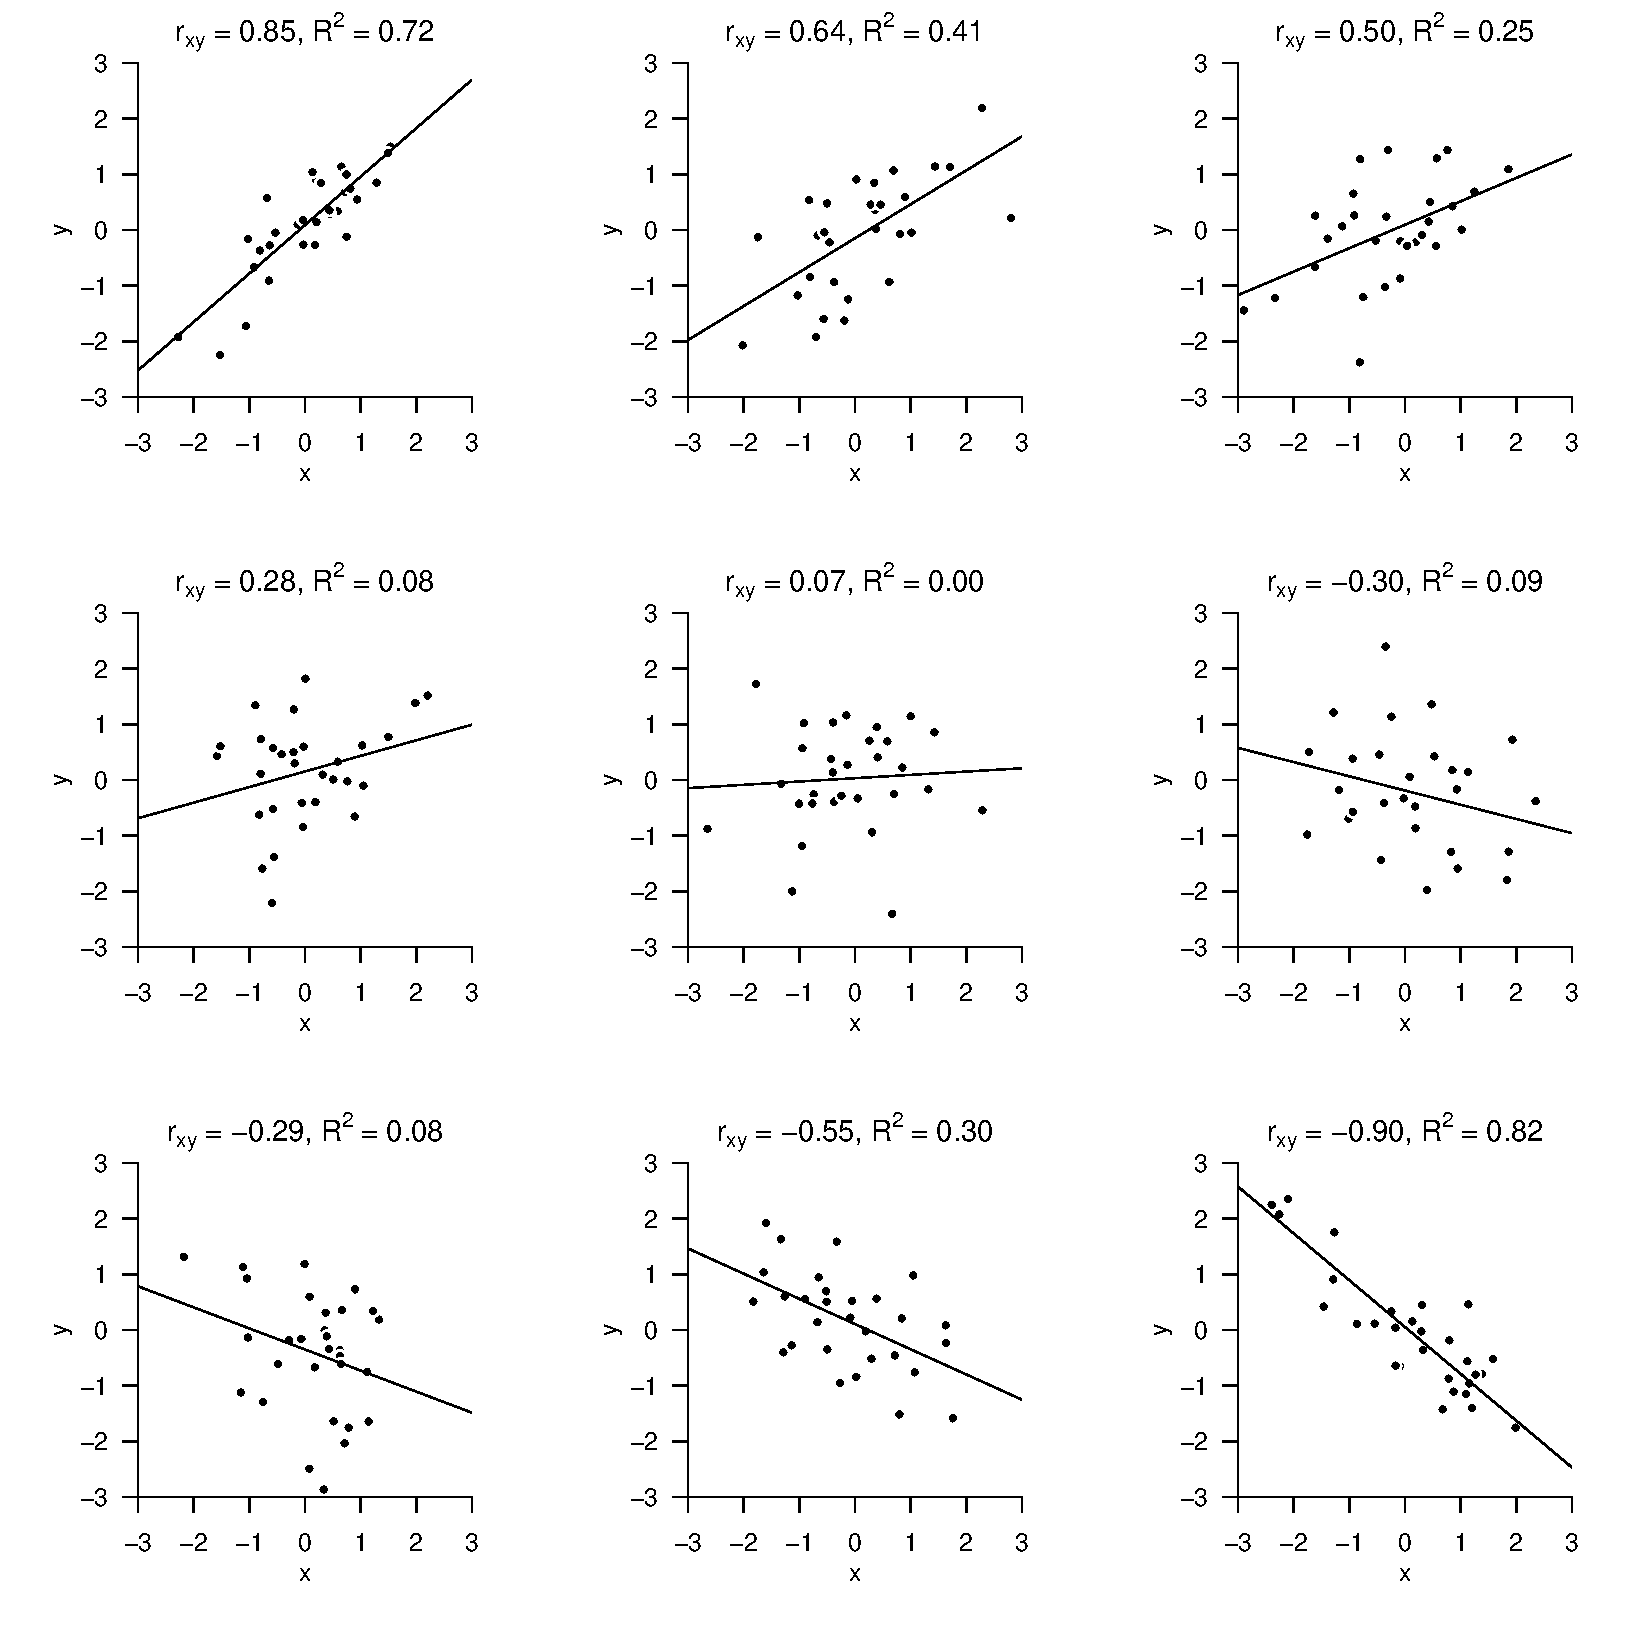
\includegraphics[width=0.6\linewidth]{2_Abbildungen/alm_2_r2beispiele} \end{center}
\end{frame}

\begin{frame}{}
\protect\hypertarget{section-5}{}
\setstretch{2}
\vfill
\large

Grundlagen

Korrelation und Bestimmtheitsmaß

\textbf{Korrelation und lineare Abhängigkeit}

Korrelation und Regression

Bedingte Korrelation und Partielle Korrelation

Selbstkontrollfragen

\vfill
\end{frame}

\begin{frame}{Korrelation und lineare Abhängigkeit}
\protect\hypertarget{korrelation-und-lineare-abhuxe4ngigkeit}{}
Funktionale Abhängigkeiten und Stichprobenkorrelation

\vspace{1cm}

\begin{center}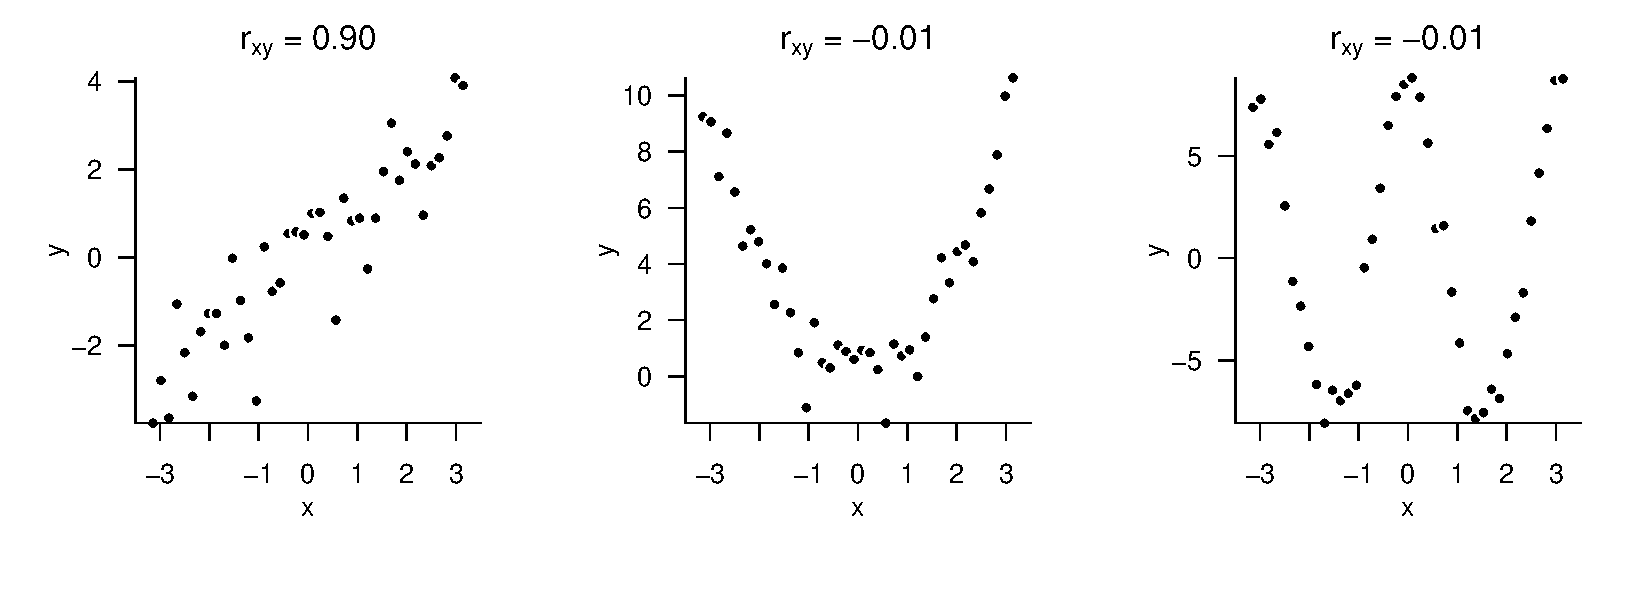
\includegraphics[width=1\linewidth]{2_Abbildungen/alm_2_rlinearitaet} \end{center}
\vspace{-5mm}

\(\,\) \hspace{1cm} \(y_i = x_i + \varepsilon_i\) \hspace{1.9cm}
\(y_i = x_i^2 + \varepsilon_i\) \hspace{1.2cm}
\(y_i = 8 \cos(2x_i) + \varepsilon_i\)

\center

\(\quad\,\,\,\varepsilon_i \sim N(0,1)\)
\end{frame}

\begin{frame}{Korrelation und lineare Abhängigkeit}
\protect\hypertarget{korrelation-und-lineare-abhuxe4ngigkeit-1}{}
\small
\begin{theorem}[Korrelation und linear-affine Abhängigkeit]
\justifying
\normalfont
$X$ und $Y$ seien zwei Zufallsvariablen mit positiver Varianz.  Dann besteht genau
dann eine lineare-affine Abhängigkeit der Form
\begin{equation}
Y = \beta_0 + \beta_1X \mbox{ mit } \beta_0,\beta_1\in \mathbb{R}
\end{equation}
zwischen $X$ und $Y$, wenn
\begin{equation}
\rho(X,Y) = 1 \mbox{ oder } \rho(X,Y) = -1
\end{equation}
gilt.
\end{theorem}

\footnotesize

Bemerkungen

\begin{itemize}
\tightlist
\item
  Die lineare Abhängigkeit \(Y = \beta_0 + \beta_1X\) impliziert eine
  lineare Abhängigkeit \(X = \tilde{\beta}_0 + \tilde{\beta}_1Y\), denn
  \begin{equation}
  Y = \beta_0 + \beta_1X
  \Leftrightarrow
  -\beta_0 + Y = \beta_1X
  \Leftrightarrow
  X = -\frac{\beta_0}{\beta_1} + \frac{1}{\beta_1}Y
  \Leftrightarrow
  X = \tilde{\beta}_0 + \tilde{\beta}_1 Y
  \end{equation} mit \begin{equation}
  \tilde{\beta}_0 = -\frac{\beta_0}{\beta_1} \mbox{ und } \tilde{\beta}_1 = \frac{1}{\beta_1}.
  \end{equation}
\end{itemize}
\end{frame}

\begin{frame}{Korrelation und lineare Abhängigkeit}
\protect\hypertarget{korrelation-und-lineare-abhuxe4ngigkeit-2}{}
\footnotesize

\underline{Beweis} \setstretch{1.0}

Wir beschränken uns auf den Beweis der Aussage, dass aus
\(Y = \beta_0 + \beta_1 X\) folgt, dass \(\rho(X,Y) = \pm 1\) ist. Dazu
halten wir zunächst fest, dass mit den Theoremen zu den Eigenschaften
von Erwartungswert und Varianz gilt, dass \begin{equation}
\mathbb{E}(Y) = \beta_0 + \beta_1\mathbb{E}(X)
\mbox{ und }
\mathbb{V}(Y) = \beta_1^2 \mathbb{V}(X).
\end{equation} Wegen \(\mathbb{V}(X) > 0\) und \(\mathbb{V}(Y) > 0\)
gilt damit \(\beta_1 \neq 0\). Es folgt dann \begin{equation}
\beta_1 > 0 \Rightarrow \mathbb{S}(Y) = \beta_1 \mathbb{S}(X) > 0
\mbox{ und }
\beta_1< 0 \Rightarrow \mathbb{S}(Y) = -\beta_1 \mathbb{S}(X) > 0.
\end{equation} Weiterhin gilt \begin{align}
\begin{split}
Y - \mathbb{E}(Y)
& = \beta_0 + \beta_1X - \mathbb{E}(Y)                      \\
& = \beta_0 + \beta_1X - \beta_0 - \beta_1\mathbb{E}(X)     \\
& = \beta_1X - \beta_1\mathbb{E}(X)                         \\
& = \beta_1(X -\mathbb{E}(X)).
\end{split}
\end{align} Für die Kovarianz von \(X\) und \(Y\) ergibt sich also
\begin{align}
\begin{split}
\mathbb{C}(X,Y)
& = \mathbb{E}\left((Y - \mathbb{E}(Y))(X - \mathbb{E}(X))\right) \\
& = \mathbb{E}\left(\beta_1(X - \mathbb{E}(X))(X - \mathbb{E}(X))\right) \\
& = \beta_1\mathbb{E}\left((X - \mathbb{E}(X))^2\right) \\
& = \beta_1\mathbb{V}(X).
\end{split}
\end{align} Damit ergibt für die Korrelation von \(X\) und \(Y\)
\begin{equation}
\rho(X,Y)
= \frac{\mathbb{C}(X,Y)}{\mathbb{S}(X)\mathbb{S}(Y)}
= \pm \frac{\beta_1\mathbb{V}(X)}{\mathbb{S}(X)\beta_1 \mathbb{S}(X)}
= \pm \frac{\beta_1\mathbb{V}(X)}{\beta_1\mathbb{V}(X)}
= \pm 1.
\end{equation}
\end{frame}

\begin{frame}{}
\protect\hypertarget{section-6}{}
\setstretch{2}
\vfill
\large

Grundlagen

Korrelation und lineare Abhängigkeit

\textbf{Korrelation und Regression}

Korrelation und Bestimmtheitsmaß

Bedingte Korrelation und Partielle Korrelation

Selbstkontrollfragen

\vfill
\end{frame}

\begin{frame}{Korrelation und Regression}
\protect\hypertarget{korrelation-und-regression}{}
Überblick

\footnotesize

Der fundamentale Unterschied zwischen ``Korrelation'' und ``Regression''
ist, dass

\begin{itemize}
\tightlist
\item
  bei Korrelation sowohl die UV (die \(x\)'s) als auch die AV (die
  \(y\)'s) als Zufallsvariablen modelliert werden,
\item
  bei Regression dagegen lediglich die AV als Zufallsvariable modelliert
  wird und die UV als vorgegeben gilt.
\end{itemize}

Dieser Tatsache unbenommen, kann man auf gegebene Daten prinzipiell
natürlich sowohl ``Korrelation'' als auch ``Regression'' anwenden. Das
Ergebnis einer Regressionsanalyse lässt sich in das Ergebnis einer
Korrelationsanalyse umrechnen. Die zusätzlich Durchführung einer
Korrelationsanalyse bei durchgeführter Regressionsanalyse erzeugt kein
mehr an Information oder Verständnis über den Zusammenhang von UV und
AV.

Für ein tieferes Verständnis dieser Zusammenhänge ist ein
Regressionsmodell nötig, indem auch die UV eine Zufallsvariable ist. In
Abgrenzung zum Modell der einfachen linearen Regression, in dem die UV
keine Zufallsvariable ist, bezeichnen wir dieses Modell als
\textit{Regression}. Letztlich gerät die Terminologie hier an eine
Grenze und es muss jeweils geprüft bzw. geschlossen werden, welches
Modell Datenanalysten nun tatsächlich vorschwebt.

Weiterhin treffen wir die Annahme, dass sowohl die UV als auch die AV im
Regressionsmodell normalverteilt sind. Diese Annahme ist nicht zwingend
nötig, da Aussagen zur Regression zweier Zufallsvariablen im
Wesentlichen die Erwartungswerte, Varianzen, und Kovarianzen berühren.
Allerdings wird die Normalverteilungsannahme für UV und AV im
Anwendungskontext häufig getroffen und bereitet didaktisch sinnvoll auf
das Konzept multivariater Normalverteilungen vor, das für die ALM
Theorie zentral ist.
\end{frame}

\begin{frame}{Korrelation und Regression}
\protect\hypertarget{korrelation-und-regression-1}{}
\footnotesize
\begin{theorem}[Bivariate Normalverteilung]
\normalfont
\justifying
$Z_1$ und $Z_2$ seien zwei standardnormalverteilte Zufallsvariablen und
$\mu_1 \in \mathbb{R},\mu_2 \in \mathbb{R}$, $\sigma_1 > 0, \sigma_2 > 0$ und
$\rho \in ]-1,1[$ seien Konstanten. Weiterhin seien $x$ und $z$ zwei Zufallsvariablen
definiert als
\begin{align}
\begin{split}
x & := \sigma_1Z_1 + \mu_1 \\
z & := \sigma_2\left(\rho Z_1 + (1-\rho^2)^{\frac{1}{2}} Z_2 \right) + \mu_2
\end{split}
\end{align}
Dann hat die gemeinsame WDF von $x$ und $z$ die Form
\begin{tiny}
\begin{multline}
p : \mathbb{R}^2 \to \mathbb{R}_{>0}, \begin{pmatrix} x \\ z \end{pmatrix} \mapsto
p\left(\begin{pmatrix} x \\ z \end{pmatrix}\right) =  \frac{1}{2\pi (1-\rho^2)^{1/2}\sigma_1\sigma_2} \\
\times \exp\left(-\frac{1}{2(1-\rho^2)}
     \left(
       \left(\frac{x - \mu}{\sigma_1}\right)^2
     - 2\rho\left(\left(\frac{x - \mu_1}{\sigma_1}\right)\left(\frac{z - \mu_2}{\sigma_2}\right)\right)
     + \left(\frac{z - \mu}{\sigma_2}\right)^2
     \right)
     \right)
\end{multline}
\end{tiny}
\end{theorem}
\end{frame}

\begin{frame}{Definition und Eigenschaften}
\protect\hypertarget{definition-und-eigenschaften}{}
\footnotesize
\begin{definition}[Korrelationsmatrix eines Zufallsvektors]
\justifying
\normalfont
$y$ sei ein $n$-dimensionaler Zufallvektor. Die \textit{Korrelationsmatrix} von
$y$ ist definiert als
\begin{equation}
\mathbb{R}(y)
= \left(\rho(y_i,y_j)\right)_{1 \le i,j \le n}
=
\begin{pmatrix}
\rho(y_1,y_1) & \rho(y_1,y_2) & \cdots & \rho(y_1,y_n) \\
\rho(y_2,y_1) & \rho(y_2,y_2) & \cdots & \rho(y_2,y_n) \\
\vdots        & \vdots        & \ddots & \vdots        \\
\rho(y_n,y_1) & \rho(y_n,y_2) & \cdots & \rho(y_n,y_n) \\
\end{pmatrix}.
\end{equation}
\end{definition}

Bemerkung

\begin{itemize}
\tightlist
\item
  Die Korrelationsmatrix \(\mathbb{R}(y)\) ist also die Matrix der
  Korrelationen der Komponenten von \(y\).
\end{itemize}
\end{frame}

\begin{frame}{Definition und Eigenschaften}
\protect\hypertarget{definition-und-eigenschaften-1}{}
\footnotesize
\begin{theorem}[Korrelationsmatrix und Kovarianzmatrix]
\justifying
\normalfont
$y$ sei ein $n$-dimensionaler Zufallvektor mit Kovarianzmatrix $\mathbb{C}(y)$.
Weiterhin sei
\begin{equation}
S_y := \mbox{diag}\left(\sqrt{\mathbb{C}(y_1,y_1)}, \sqrt{\mathbb{C}(y_2,y_2)}, ...,\sqrt{\mathbb{C}(y_n,y_n)}\right)
\end{equation}
die Diagonalmatrix der Standardabweichungen er Komponenten von $y$. Dann gelten
\begin{equation}
\mathbb{R}(y)
= S_y^{-1}\mathbb{C}(y)S_y^{-1}
\end{equation}
und
\begin{equation}
\mathbb{C}(y)
= S_y\mathbb{R}(y)S_y
\end{equation}
\end{theorem}

Bemerkungen

\begin{itemize}
\tightlist
\item
  \(\mathbb{C}(y)\) kann mithilfe ihrer Diagonalelemente in
  \(\mathbb{R}(y)\) umgerechnet werden.
\item
  \(\mathbb{R}(y)\) kann mithilfe der Diagonalelemente von
  \(\mathbb{C}(y)\) in \(\mathbb{C}(y)\) umgerechnet werden.
\item
  \(\mathbb{C}(y)\) enthält also mehr Information als \(\mathbb{R}(y)\).
\end{itemize}
\end{frame}

\begin{frame}{Definition und Eigenschaften}
\protect\hypertarget{definition-und-eigenschaften-2}{}
\footnotesize

\underline{Beweis}

Wir halten zunächst fest, dass \begin{equation}
S^{-1}_y = \mbox{diag}\left(\frac{1}{\sqrt{\mathbb{C}(y_1,y_1)}}, \frac{1}{\sqrt{\mathbb{C}(y_2,y_2)}}, ...,\frac{1}{\sqrt{\mathbb{C}(y_n,y_n)}}\right)
\end{equation} Es ergibt sich dann \begin{align}
\begin{split}
S_y^{-1}\mathbb{C}(y)S_y^{-1}
& = \left(\frac{\mathbb{C}(y_i,y_j)}{\sqrt{\mathbb{C}(y_i,y_i)}}\right)_{1 \le i,j \le n}S_y^{-1} \\
& = \left(\frac{\mathbb{C}(y_i,y_j)}{\sqrt{\mathbb{C}(y_i,y_i)}\sqrt{\mathbb{C}(y_j,y_j)}}\right)_{1 \le i,j \le n} \\
& = \left(\rho(y_i,y_j)\right)_{1 \le i,j \le n} \\
& =: \mathbb{R}(y) \\
\end{split}
\end{align}
\end{frame}

\begin{frame}{Definition und Eigenschaften}
\protect\hypertarget{definition-und-eigenschaften-3}{}
\footnotesize

\underline{Beweis}

Analog ergibt sich \begin{align}
\begin{split}
S_y\mathbb{R}(y)S_y
& = \left(\frac{\sqrt{\mathbb{C}(y_i,y_i)}\mathbb{C}(y_i,y_j)}{\sqrt{\mathbb{C}(y_i,y_i)}\sqrt{\mathbb{C}(y_j,y_j)}}\right)_{1 \le i,j \le n} S_y\\
& = \left(\frac{\mathbb{C}(y_i,y_j)\sqrt{\mathbb{C}(y_j,y_j)}}{\sqrt{\mathbb{C}(y_j,y_j)}}\right)_{1 \le i,j \le n}\\
& = \left(\mathbb{C}(y_i,y_j)\right)_{1 \le i,j \le n}\\
& =: \mathbb{C}(y). \\
\end{split}
\end{align}
\end{frame}

\begin{frame}{Definition und Eigenschaften}
\protect\hypertarget{definition-und-eigenschaften-4}{}
\footnotesize
\begin{theorem}[Korrelationsmatrix eines normalverteilten Zufallsvektors]
\justifying
\normalfont
$y \sim N(\mu,\Sigma)$ sei ein multivariat normalverteilter Zufallsvektor mit
Erwartungswertparameter $\mu \in \mathbb{R}^n$ und Kovarianzmatrixparameter
\begin{equation}
\Sigma
:= \left(\sigma_{ij}^2\right)_{1 \le i,j \le n}
=
\begin{pmatrix}
\sigma_{11}^2  & \sigma_{12}^2  & \cdots &  \sigma_{1n}^2 \\
\sigma_{21}^2  & \sigma_{22}^2  & \cdots &  \sigma_{2n}^2 \\
\vdots         & \vdots         & \ddots &  \vdots        \\
\sigma_{n1}^2  & \sigma_{n2}^2  & \cdots &  \sigma_{nn}^2 \\
\end{pmatrix}
\in \mathbb{R}^{n \times n}\mbox{p.d.}.
\end{equation}
Dann gilt
\begin{equation}
\renewcommand{\arraystretch}{1.5}
\mathbb{R}(y)
= \left(\frac{\sigma_{ij}^2}{\sigma_{ii}\sigma_{jj}}\right)_{1 \le i,j \le n}
=
\begin{pmatrix}
1
& \frac{\sigma_{12}^2}{\sigma_{11}\sigma_{22}}
& \cdots
& \frac{\sigma_{1n}^2}{\sigma_{11}\sigma_{nn}}
\\
  \frac{\sigma_{21}^2}{\sigma_{22}\sigma_{11}}
&  1
& \cdots
& \frac{\sigma_{2n}^2}{\sigma_{22}\sigma_{nn}}
\\
\vdots
& \vdots
& \ddots
& \vdots
\\
  \frac{\sigma_{n1}^2}{\sigma_{nn}\sigma_{11}}
& \frac{\sigma_{n2}^2}{\sigma_{nn}\sigma_{22}}
& \cdots
& 1
\end{pmatrix}.
\end{equation}
\end{theorem}

Bemerkungen

\begin{itemize}
\tightlist
\item
  Das Theorem folgt direkt mit dem Theorem zu Korrelationsmatrix und
  Kovarianzmatrix
\end{itemize}
\end{frame}

\begin{frame}{Definition und Eigenschaften}
\protect\hypertarget{definition-und-eigenschaften-5}{}
\footnotesize

Bemerkungen (fortgeführt)

\begin{itemize}
\tightlist
\item
  Umgekehrt gilt bei Definition eines Korrelationsmatrixparameters
  \begin{equation}
  R
  := \left(\rho_{ij}\right)_{1 \le i,j \le 1}
  =
  \begin{pmatrix}
  \rho_{11}
  & \rho_{12}
  & \cdots
  & \rho_{1n}
  \\
  \rho_{21}
  & \rho_{22}
  & \cdots
  & \rho_{2n}
  \\
  \vdots
  & \vdots
  & \ddots
  & \vdots
  \\
  \rho_{n1}
  & \rho_{n2}
  & \cdots
  & \rho_{nn}
  \end{pmatrix}
  \end{equation} mit \begin{equation}
  \rho_{ij} := 1 \mbox{ für } i = j
  \mbox{ und }
  \rho_{ij} = \rho_{ji} \in ]-1,1[ \mbox{ für } i \neq j
  \mbox{ für } 1 \le i,j \le n
  \end{equation} und zusätzlicher Definition von \begin{equation}
  S_{y} := \mbox{diag}(\sigma_{11}, ...,\sigma_{nn})
  \mbox{ mit } \sigma_{11},...,\sigma_{nn} > 0,
  \end{equation} dass \begin{equation}
  \Sigma
  := S_y R S_y
  = \begin{pmatrix}
  \sigma_{11}\sigma_{11}
  & \rho_{12}\sigma_{11}\sigma_{22}
  & \cdots
  & \rho_{1n}\sigma_{11}\sigma_{nn}
  \\
  \rho_{21}\sigma_{22}\sigma_{11}
  & \sigma_{22}\sigma_{22}
  & \cdots
  & \rho_{2n}\sigma_{22}\sigma_{nn}
  \\
  \vdots
  & \vdots
  & \ddots
  & \vdots
  \\
  \rho_{n1}\sigma_{nn}\sigma_{11}
  & \rho_{n2}\sigma_{nn}\sigma_{22}
  & \cdots
  & \sigma_{nn}\sigma_{nn}
  \end{pmatrix}
  \end{equation} einen Kovarianzmatrixparameter eines multivariate
  normalverteilten Zufallsvektors definiert.
\end{itemize}
\end{frame}

\begin{frame}{Korrelation und Regression}
\protect\hypertarget{korrelation-und-regression-2}{}
\small
\begin{definition}[Regressionsgerade zweier Zufallsvariablen]
\justifying
$X$ und $Y$ seien zwei Zufallsvariablen. Dann heißt
\begin{equation}
Y  = \beta_0 + \beta_1 X \mbox{ mit }
\end{equation}
mit
\begin{equation}
\beta_1 := \frac{\mathbb{C}(X,Y)}{\mathbb{V}(X)} \mbox{ und }\beta_0 := \mathbb{E}(Y) - \beta_1\mathbb{E}(X)
\end{equation}
die \textit{Regressionsgerade der Zufallsvariablen $X$ auf $Y$}, $\beta_0$ und
$\beta_1$ heißen die zugehörigen \textit{Regressionskoeffizienten}, und die
Zufallsvariable
\begin{equation}
E := Y - \beta_0 - \beta_1 X
\end{equation}
heißt die \textit{Residualvariable}.
\end{definition}

\footnotesize

Bemerkungen

\begin{itemize}
\tightlist
\item
  \(X\) und \(Y\) sind Zufallsvariablen, \(\beta_0\) und \(\beta_1\)
  sind keine Zufallsvariablen.
\end{itemize}
\end{frame}

\begin{frame}{Korrelation und Regression}
\protect\hypertarget{korrelation-und-regression-3}{}
\small
\begin{theorem}[Optimalität der Regressionsgerade zweier Zufallsvariablen]
\justifying
\normalfont
Unter allen Geraden der Form
\begin{equation}
Y  = \beta_0 + \beta_1 X
\end{equation}
ist die Gerade mit
\begin{equation}
\beta_1 := \frac{\mathbb{C}(X,Y)}{\mathbb{V}(X)} \mbox{ und } \beta_0 :=  \mathbb{E}(Y) - \beta_1\mathbb{E}(X)
\end{equation}
diejenige, für die
\begin{equation}
\tilde{q}: \mathbb{R}^2 \to \mathbb{R}, (\beta_0, \beta_1) \mapsto \tilde{q}(\beta_0,\beta_1) := \mathbb{E}\left((Y - (\beta_0 + \beta_1 X)^2\right)
\end{equation}
ein Minimum hat.
\end{theorem}
\end{frame}

\begin{frame}{Korrelation und Regression}
\protect\hypertarget{korrelation-und-regression-4}{}
\tiny
\setstretch{1}
\tiny
\setlength{\abovedisplayskip}{3pt}
\setlength{\belowdisplayskip}{3pt}

\underline{Beweis}

Wir halten zunächst fest, dass \begin{align}
\begin{split}
\tilde{q}(\beta_0,\beta_1)
& = \mathbb{E}\left(Y - \beta_0 - \beta_1 X \right) \\
& = \mathbb{E}\left(Y - \beta_1 X - \beta_0 + \beta\mathbb{E}(X) - \beta_1\mathbb{E}(X) + \mathbb{E}(Y) - \mathbb{E}(Y) \right) \\
& = \mathbb{E}\left((Y - \mathbb{E}(Y)) - \beta_1(X - \mathbb{E}(X)) + (\mathbb{E}(Y) - \beta_1\mathbb{E}(X) - \beta_0)\right) \\
\end{split}
\end{align} Ausmultiplizieren und Anwendung des Theorems zu den
Eigenschaften des Erwartungswerts ergibt dann \begin{equation}
\tilde{q}(\beta_0,\beta_1) = \mathbb{V}(Y) + \beta_1^2 \mathbb{V}(X) - 2 \beta_1 \mathbb{C}(X,Y) + \left(\mathbb{E}(Y) - \beta_1 \mathbb{E}(X) - \beta_0\right)^2
\end{equation} Berechnen der partiellen Ableitungen von \(\tilde{q}\)
hinsichtlich von \(\beta_0\) und \(\beta_1\) ergibt dann
\begin{equation}\label{eq:partial_beta_0}
\frac{\partial}{\partial \beta_0}\tilde{q}(\beta_0,\beta_1) = -2\left(\mathbb{E}(Y) - \beta_1 \mathbb{E}(X) - \beta_0\right)
\end{equation} und \begin{equation}
\frac{\partial}{\partial \beta_1}\tilde{q}(\beta_0,\beta_1) = 2\beta_1\mathbb{V}(X) - 2\mathbb{C}(X,Y) - 2\mathbb{E}(X)\left(\mathbb{E}(Y) - \beta_1\mathbb{E} - \beta_0\right)
\end{equation} Nullsetzen von \eqref{eq:partial_beta_0} ergibt dann als
notwendige Bedingungen für ein Minimum von \(\tilde{q}\) \begin{align}
\begin{split}
\frac{\partial}{\partial \beta_0}\tilde{q}(\beta_0^*,\beta_1^*)     = 0
& \Leftrightarrow
\mathbb{E}(Y) - \beta_1^* \mathbb{E}(X) - \beta_0^* = 0 \\
\frac{\partial}{\partial \beta_1}\tilde{q}(\beta_0^*,\beta_1*)  = 0
& \Leftrightarrow
2\beta_1^*\mathbb{V}(X) - 2\mathbb{C}(X,Y) - 2\mathbb{E}(X)\left(\mathbb{E}(Y) - \beta_1^*\mathbb{E} - \beta_0^*\right) = 0
\end{split}
\end{align} Die erste Gleichung impliziert dann für die zweite
Gleichung, dass \begin{equation}
2\beta_1^*\mathbb{V}(X) - 2\mathbb{C}(X,Y) = 0 \Leftrightarrow \beta_1^* = \frac{\mathbb{C}(X,Y)}{\mathbb{V}(X)}
\end{equation} Einsetzen in die erste Gleichung ergibt dann
\begin{align}
\begin{split}
\mathbb{E}(Y) - \beta_1^* \mathbb{E}(X) - \beta_0^* & = 0
\Leftrightarrow
\beta_0^*   = \mathbb{E}(Y) - \beta_1^* \mathbb{E}(X) \\
\end{split}
\end{align}
\end{frame}

\begin{frame}{Korrelation und Regression}
\protect\hypertarget{korrelation-und-regression-5}{}
\footnotesize
\begin{theorem}[Zusammenhang von Korrelation und Regression]
\normalfont
\justifying
$X$ und $Y$ seien zwei Zufallsvariablen,
\begin{equation}
Y = \beta_0 + \beta_1 X
\mbox{ mit }
\beta_1 := \frac{\mathbb{C}(X,Y)}{\mathbb{V}(X)}
\mbox{ und }
\beta_0 := \mathbb{E}(Y) -\tilde{\beta}_1\mathbb{E}(X)
\end{equation}
sei die Regressionsgerade der Zufallsvariablen $Y$ bezüglich der Zufallsvariablen
$X$ mit den Regressionskoeffizienten  $\beta_0$ und $\beta_1$ und
\begin{equation}
X = \tilde{\beta}_0 + \tilde{\beta_1} Y
\mbox{ mit }
\tilde{\beta}_1 := \frac{\mathbb{C}(X,Y)}{\mathbb{V}(Y)}
\mbox{ und }
\tilde{\beta}_0 := \mathbb{E}(X) -\tilde{\beta}_1\mathbb{E}(Y)
\end{equation}
sei die Regressionsgerade der Zufallsvariablen $X$ bezüglich der Zufallsvariablen
$Y$ mit den Regressionskoeffizienten $\tilde{\beta}_0$ und $\tilde{\beta}_1$. Dann gilt
\begin{equation}
\beta_1 \tilde{\beta}_1
= \frac{\mathbb{C}(X,Y)}{\mathbb{V}(X)}\frac{\mathbb{C}(X,Y)}{\mathbb{V}(Y)}
= \frac{\mathbb{C}(X,Y)^2}{\mathbb{V}(X)\mathbb{V}(Y)}
= \rho(X,Y)^2.
\end{equation}
\end{theorem}

Bemerkungen

\begin{itemize}
\tightlist
\item
  \(\rho(X,Y)\) kann aus den Regressionskoeffizienten von \(X\) auf
  \(Y\) und von \(Y\) auf \(X\) errechnet werden.
\end{itemize}
\end{frame}

\begin{frame}{Korrelation und Regression}
\protect\hypertarget{korrelation-und-regression-6}{}
\footnotesize
\begin{definition}[Stichprobenregressionsgerade]
\justifying
$(x,Y_1), ..., (X_n,Y_n)$ sei eine Stichprobe von zweidimensionale Zufallsvektoren
mit identischen unabhängigen Verteilungen. Weiterhin sei für $i = 1,...,n$
\begin{equation}
Y_1 = \beta_0 + \beta_1 x
\mbox{ mit }
\beta_1 := \frac{\mathbb{C}(x,Y_1)}{\mathbb{V}(x)}
\mbox{ und }
\beta_0 := \beta_1\mathbb{E}(x) + \mathbb{E}(Y_1)
\end{equation}
die Regressionsgerade der Zufallsvariablen $Y_1$ bezüglich der Zufallsvariablen
$x$ mit den Regressionskoeffizienten  $\beta_0$ und $\beta_1$. Schließlich seien
\begin{itemize}
\item $\bar{x}$  und $\bar{y}$ die Stichprobenmittel von Realisierungen der Komponenten der Stichprobe,
\item $s_X^2$ und $s_Y^2$ die Stichprobenvarianzen von Realisierungen der Komponenten der Stichprobe und
\item $c_{X,Y}$ die Stichprobenkovarianz  von Realisierungen der Stichprobe.
\end{itemize}
Dann heißt für $x \in \mathbb{R}$
\begin{equation}
y = b_0 + b_1 x
\mbox{ mit }
b_1 := \frac{c_{X,Y}}{s_X^2}
\mbox{ und }
b_0 := \bar{y} - b_1\bar{x}
\end{equation}
die Regressionsgerade der $y$-Werte bezüglich der $x_i$ Werte in der Stichprobe.
\end{definition}
\end{frame}

\begin{frame}[fragile]{Korrelation und Regression}
\protect\hypertarget{korrelation-und-regression-7}{}
Simulation einer Regressionsgerade

\tiny
\setstretch{1}

\begin{Shaded}
\begin{Highlighting}[]
\FunctionTok{library}\NormalTok{(MASS)                                   }\CommentTok{\# multivariate Normalverteilungen}

\CommentTok{\# Modellformulierung}
\NormalTok{n      }\OtherTok{=} \FloatTok{1e2}                                     \CommentTok{\# Anzahl an Stichprobenvektoren}
\NormalTok{C\_XY   }\OtherTok{=} \DecValTok{1}                                      \CommentTok{\# Kovarianz von X und Y}
\NormalTok{EX     }\OtherTok{=} \DecValTok{2}                                      \CommentTok{\# Erwartungswert von X}
\NormalTok{EY     }\OtherTok{=} \DecValTok{1}                                      \CommentTok{\# Erwartungswert von Y}
\NormalTok{VX     }\OtherTok{=} \DecValTok{2}                                      \CommentTok{\# Varianz von X}
\NormalTok{VY     }\OtherTok{=} \DecValTok{2}                                      \CommentTok{\# Varianz von Y}
\NormalTok{beta\_1 }\OtherTok{=}\NormalTok{ C\_XY}\SpecialCharTok{/}\NormalTok{VX                                }\CommentTok{\# Regressionskoeffizient}
\NormalTok{beta\_0 }\OtherTok{=} \SpecialCharTok{{-}}\NormalTok{beta\_1}\SpecialCharTok{*}\NormalTok{EX }\SpecialCharTok{+}\NormalTok{ EY                        }\CommentTok{\# Regressionskoeffizient}

\CommentTok{\# Realisierungsgeneration}
\NormalTok{mu     }\OtherTok{=} \FunctionTok{c}\NormalTok{(EX, EY)                              }\CommentTok{\# Erwartungswertparameter}
\NormalTok{Sigma  }\OtherTok{=} \FunctionTok{matrix}\NormalTok{(}\FunctionTok{c}\NormalTok{(VX, C\_XY, C\_XY,VY), }\AttributeTok{nrow =} \DecValTok{2}\NormalTok{) }\CommentTok{\# Kovarianzmatrixparameter}
\NormalTok{xy     }\OtherTok{=} \FunctionTok{mvrnorm}\NormalTok{(n, mu, Sigma)}

\CommentTok{\# Stichprobenstatistiken}
\NormalTok{x\_bar  }\OtherTok{=} \FunctionTok{mean}\NormalTok{(xy[,}\DecValTok{1}\NormalTok{])                           }\CommentTok{\# Stichprobenmittel  der x,...,x\_n}
\NormalTok{y\_bar  }\OtherTok{=} \FunctionTok{mean}\NormalTok{(xy[,}\DecValTok{2}\NormalTok{])                           }\CommentTok{\# Stichprobenmittel  der y\_1,...,y\_n}
\NormalTok{s2X    }\OtherTok{=} \FunctionTok{var}\NormalTok{(xy[,}\DecValTok{1}\NormalTok{])                            }\CommentTok{\# Stichprobenvarianz der x,...,x\_n}
\NormalTok{s2Y    }\OtherTok{=} \FunctionTok{var}\NormalTok{(xy[,}\DecValTok{2}\NormalTok{])                            }\CommentTok{\# Stichprobenvarianz der y\_1,...,y\_n}
\NormalTok{c\_xy   }\OtherTok{=} \FunctionTok{cov}\NormalTok{(xy[,}\DecValTok{1}\NormalTok{],xy[,}\DecValTok{2}\NormalTok{])                     }\CommentTok{\# Stichprobenkovarianz}

\CommentTok{\# Stichprobenregressionsgeradenparameter}
\NormalTok{b\_1    }\OtherTok{=}\NormalTok{ c\_xy}\SpecialCharTok{/}\NormalTok{s2X                               }\CommentTok{\# Stichprobenregressionskoeffizient}
\NormalTok{b\_0    }\OtherTok{=} \SpecialCharTok{{-}}\NormalTok{b\_1}\SpecialCharTok{*}\NormalTok{x\_bar }\SpecialCharTok{+}\NormalTok{ y\_bar                     }\CommentTok{\# Stichprobenregressionskoeffizient}
\end{Highlighting}
\end{Shaded}

\begin{verbatim}
> beta_0   : 0 
> beta_1   : 0.5 
> b_0      : 0.136 
> b_1      : 0.514
\end{verbatim}
\end{frame}

\begin{frame}{Korrelation und Regression}
\protect\hypertarget{korrelation-und-regression-8}{}
Simulation einer Regressionsgerade \vspace{3mm}

\begin{center}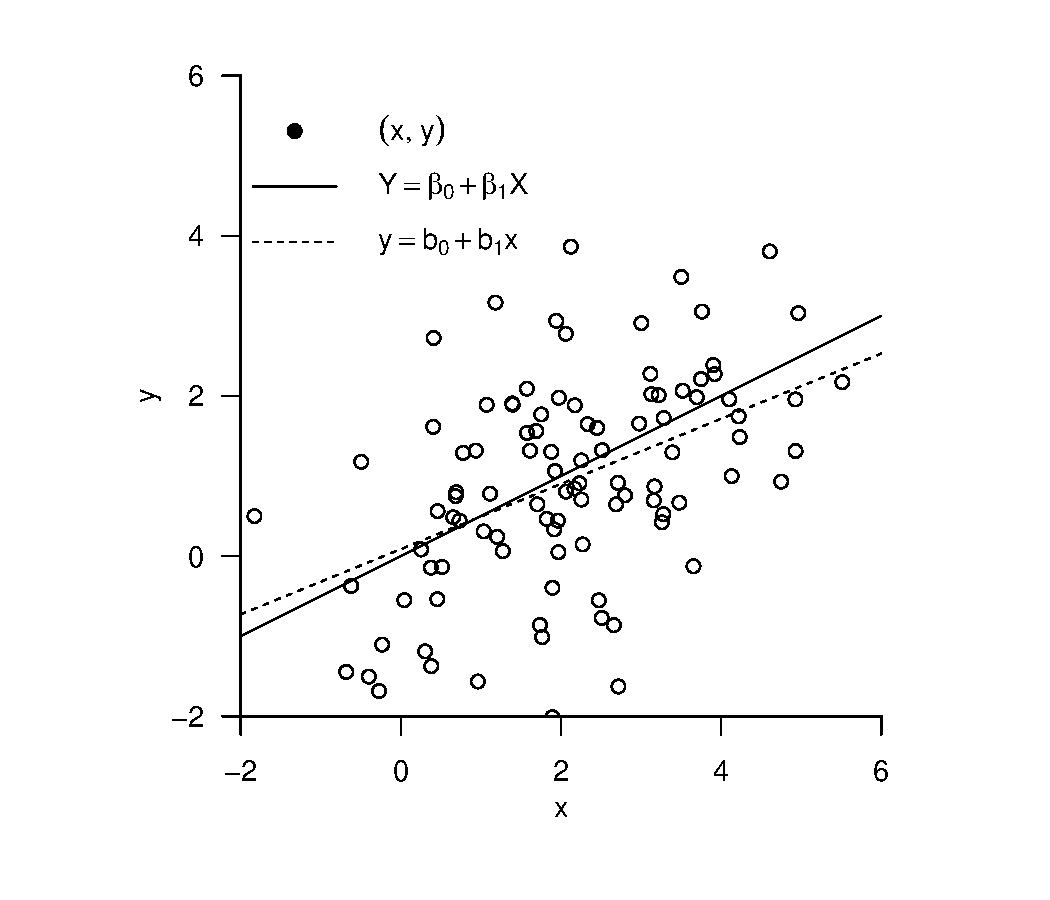
\includegraphics[width=0.6\linewidth]{2_Abbildungen/alm_2_stichprobenregression} \end{center}
\end{frame}

\begin{frame}{}
\protect\hypertarget{section-7}{}
\setstretch{2}
\vfill
\large

Grundlagen

Korrelation und lineare Abhängigkeit

Korrelation und Regression

Korrelation und Bestimmtheitsmaß

\textbf{Bedingte Korrelation und Partielle Korrelation}

Selbstkontrollfragen

\vfill
\end{frame}

\begin{frame}{Bedingte Korrelation und Partielle Korrelation}
\protect\hypertarget{bedingte-korrelation-und-partielle-korrelation}{}
\center

\textcolor{darkblue}{Jährlicher Eiskonsum und jährliche Sonnenbrandinzidenz}

\begin{center}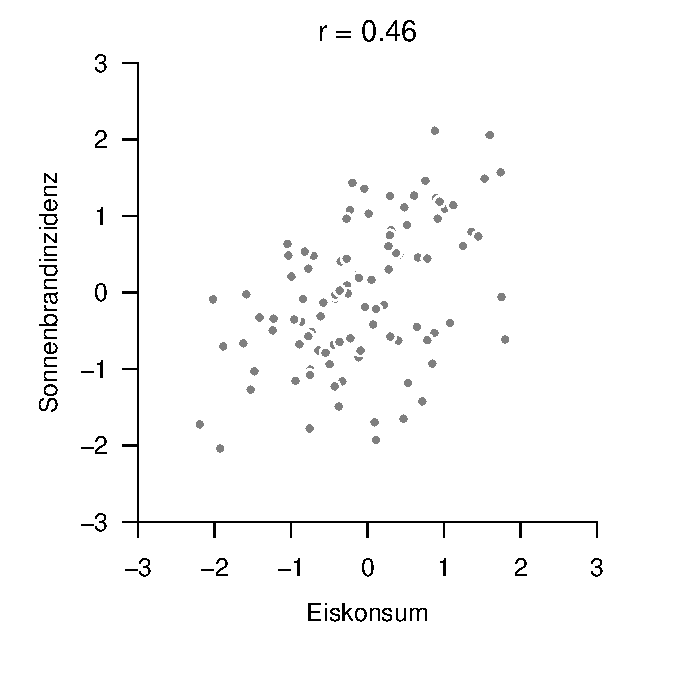
\includegraphics[width=0.5\linewidth]{2_Abbildungen/alm_2_bpr_beispiel} \end{center}
\small
\vspace{-2mm}

\begin{itemize}
\tightlist
\item
  Korrelation impliziert keine Kausalität.
\item
  Kausalität wird zumeist als Koinzidenz mit zeitlicher Rangefolge
  modelliert.
\item
  Einstiege in die kausale Inferenz geben z.B. Pearl (2000) und Imbens
  and Rubin (2015).
\end{itemize}
\end{frame}

\begin{frame}{Bedingte Korrelation und Partielle Korrelation}
\protect\hypertarget{bedingte-korrelation-und-partielle-korrelation-1}{}
\center

\textcolor{darkblue}{Jährlicher Eiskonsum und jährliche Sonnenbrandinzidenz}
\vspace{2mm}

\begin{center}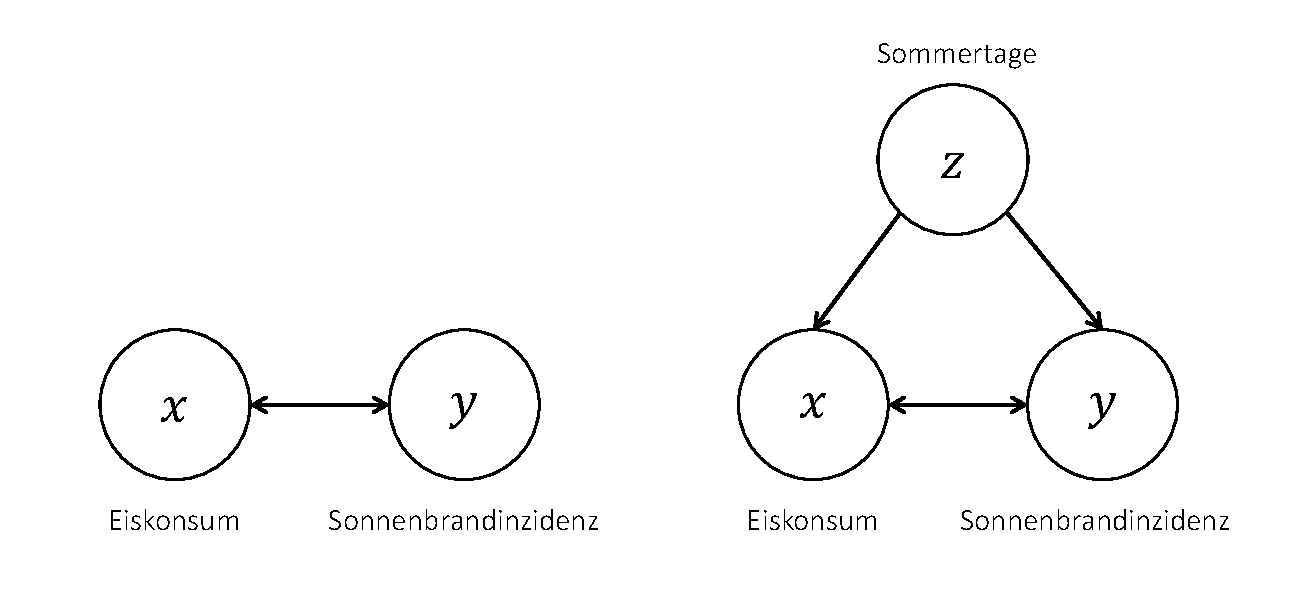
\includegraphics[width=0.8\linewidth]{2_Abbildungen/alm_2_eis_sonnenbrand_sommer} \end{center}

\small

\begin{itemize}
\tightlist
\item
  Korrelation von Eiskonsum und Sonnenbrandinzidenz nach Korrektur für
  Sommertage?
\item
  ``Herausrechnen'' des Einflusses von \(z\) auf die Kovariation von
  \(x\) und \(y\)?
\end{itemize}

\center
\normalsize

\textcolor{darkblue}{$\Rightarrow$ Bedingte Korrelation und Partielle Korrelation im Falle dreier Zufallsvariablen.}
\end{frame}

\begin{frame}{Bedingte Korrelation und Partielle Korrelation}
\protect\hypertarget{bedingte-korrelation-und-partielle-korrelation-2}{}
\footnotesize
\begin{definition}[Bedingte Kovarianz und bedingte Korrelation]
\justifying
Gegeben seien drei Zufallsvariablen $x,y,z$ einer gemeinsamen Verteilung
$\mathbb{P}_{x,y,z}(x,y,z)$.  Weiterhin sei $\mathbb{P}_{x,y |z}(x,y)$ 
die bedingte Verteilung von $x$ und $y$ gegeben $z$. Dann heißt
die Kovarianz von $x$ und $y$ in der Verteilung $\mathbb{P}_{x,y|z}(x,y)$
die \textit{bedingte Kovarianz von $x$ und $y$ gegeben $z$} und
wird mit $\mathbb{C}(x,y|z)$ bezeichnet. Weiterhin seien $\mathbb{P}_{x,y|z}(y)$ und 
$\mathbb{P}_{x,y|z}(x)$ die marginalen Verteilungen von $x$ und $y$ gegeben $z$, 
respektive, und $\mathbb{S}(x|z)$, $\mathbb{S}(y|z)$
die Standardabweichungen von $x$ und $y$ hinsichtlich
$\mathbb{P}_{x,y|z}(y)$  und $\mathbb{P}_{x,y|z}(x)$, respektive. 
Dann heißt die Korrelation von $x$ und $y$ in der Verteilung $\mathbb{P}_{x,y|z}(x,y)$,
\begin{equation}
\rho(x,y|z) := \frac{\mathbb{C}(x,y|z)}{\mathbb{S}(y  |z)\mathbb{S}(x|z)}
\end{equation}
die \textit{bedingte Korrelation von $x$ und $y$ gegeben $z$}
\end{definition}

Bemerkungen

\begin{itemize}
\tightlist
\item
  Die bedingte Kovarianz zweier ZVen ist die Kovarianz zweier ZVen in
  einer bedingten Verteilung
\item
  Die bedingte Korrelation zweier ZVen ist die Korrelation zweier ZVen
  in einer bedingten Verteilung.
\item
  Durch Vertauschen der Variablennamen kann man analog \(\rho(y,z|x)\)
  und \(\rho(x,z|y)\) definieren.
\end{itemize}
\end{frame}

\begin{frame}{Bedingte Korrelation und Partielle Korrelation}
\protect\hypertarget{bedingte-korrelation-und-partielle-korrelation-3}{}
\vspace{1mm}
\small

\textcolor{darkblue}{Beispiel} \footnotesize

Die Zufallsvariablen \(x,y,z\) seien multivariat normalverteilt. Wir
wollen die bedingte Korrelation von \(x\) und \(y\) gegeben \(z\)
bestimmen. Für \(v := (x,y,z)^T\) gelte also, dass \begin{equation}
v\sim N(\mu,\Sigma)
\end{equation} mit \begin{equation}
\mu
:=
\begin{pmatrix*}[l]
\mu_y     \\
\mu_{x} \\
\mu_{z}
\end{pmatrix*}
\mbox{ und }
\Sigma :=
\begin{pmatrix*}[l]
\sigma^2_{x}   & \sigma^2_{x,y} & \sigma^{2}_{x,z} \\
\sigma^2_{y,x} & \sigma^2_{y}   & \sigma^{2}_{y,z} \\
\sigma^2_{z,x} & \sigma^2_{z,y} & \sigma^{2}_{z}     \\
\end{pmatrix*}
\end{equation} Um die Kovarianzmatrix der bedingten Verteilung von \(x\)
und \(y\) gegeben \(z\) zu bestimmenm definieren wir zunächst
\begin{equation}
\Sigma_{x,y}
:=
\begin{pmatrix*}[l]
\sigma^2_{x}   & \sigma^2_{x,y} \\
\sigma^2_{y,x} & \sigma^2_{y}
\end{pmatrix*},
\Sigma_{z}
:=
\begin{pmatrix*}[l]
\sigma^{2}_{z}
\end{pmatrix*}
\mbox{ und }
\Sigma_{(x,y),z} := \Sigma_{z, (x,y)}^T :=
\begin{pmatrix*}[l]
\sigma^{2}_{x,z} \\
\sigma^{2}_{y,z} \\
\end{pmatrix*},
\end{equation} so dass \begin{equation}
\Sigma =
\begin{pmatrix}
\Sigma_{x,y}      & \Sigma_{(x,y),z} \\
\Sigma_{z, (x,y)} & \Sigma_{z}
\end{pmatrix}
\end{equation} Mit dem Theorem zu bedingten Normalverteilungen (vgl. (4)
Normalverteilungen) ist dann die Kovarianzmatrix des Zufallsvektors
\((x,y)\) gegeben durch \begin{equation}
\Sigma_{x,y|z}
= \Sigma_{x,y} - \Sigma_{(x,y),z}\Sigma_{z}^{-1}\Sigma_{z,(x,y)}.
\end{equation}
\end{frame}

\begin{frame}{Bedingte Korrelation und Partielle Korrelation}
\protect\hypertarget{bedingte-korrelation-und-partielle-korrelation-4}{}
\small
\vspace{1mm}

\textcolor{darkblue}{Beispiel (fortgeführt)} \footnotesize

Mit den Eigenschaften der multivariaten Normalverteilung gilt dann, dass
die die Diagonaleinträge von \(\Sigma_{x,y|z}\) den bedingten Varianzen
von \(x\) und \(y\) gegeben \(z\) entsprechen und dass der
Nichtdiagonaleintrag die bedingte Kovarianz von \(x\) und \(y\) gegeben
\(z\) ist. In anderen Worten gilt \begin{equation}
\Sigma_{x,y|z} =
\begin{pmatrix}
\mathbb{C}(x,x|z) & \mathbb{C}(x,y|z)   \\
\mathbb{C}(y,x|z) & \mathbb{C}(y,y|z)   \\
\end{pmatrix}.
\end{equation} Die bedingte Korrelation \(\rho(x,y|z)\) von \(x\) und
\(y\) gegeben \(z\) ergibt sich dann aus den Einträgen von
\(\Sigma_{x,y|z}\) gemäß \begin{equation}
\rho(x,y|z) = \frac{\mathbb{C}(x,y|z)}{\sqrt{\mathbb{C}(x,x|z)}\sqrt{\mathbb{C}(y,y|z)}}
\end{equation} Für \begin{equation}
\Sigma :=
\begin{pmatrix}
1.0 & 0.5 & 0.9 \\
0.5 & 1.0 & 0.5 \\
0.9 & 0.5 & 1.0 \\
\end{pmatrix}
\end{equation} ergibt sich beispielsweise \begin{equation}
\rho(x,y) = 0.50 \mbox{ und } \rho(x,y|z) \approx 0.13.
\end{equation}
\end{frame}

\begin{frame}[fragile]{Bedingte Korrelation und Partielle Korrelation}
\protect\hypertarget{bedingte-korrelation-und-partielle-korrelation-5}{}
\small
\vspace{1mm}

\textcolor{darkblue}{Beispiel (fortgeführt)} \footnotesize \vspace{2mm}

\begin{Shaded}
\begin{Highlighting}[]
\CommentTok{\# Bedingte Korrelation bei Normalverteilung }
\NormalTok{S         }\OtherTok{=} \FunctionTok{matrix}\NormalTok{(}\FunctionTok{c}\NormalTok{( }\DecValTok{1}\NormalTok{,.}\DecValTok{5}\NormalTok{,.}\DecValTok{9}\NormalTok{,                                   }\CommentTok{\# \textbackslash{}Sigma}
\NormalTok{                     .}\DecValTok{5}\NormalTok{, }\DecValTok{1}\NormalTok{,.}\DecValTok{5}\NormalTok{,}
\NormalTok{                     .}\DecValTok{9}\NormalTok{,.}\DecValTok{5}\NormalTok{, }\DecValTok{1}\NormalTok{), }\AttributeTok{nrow  =} \DecValTok{3}\NormalTok{, }\AttributeTok{byrow =} \ConstantTok{TRUE}\NormalTok{)}
\NormalTok{rho\_xy    }\OtherTok{=}\NormalTok{ S[}\DecValTok{1}\NormalTok{,}\DecValTok{2}\NormalTok{]}\SpecialCharTok{/}\NormalTok{(}\FunctionTok{sqrt}\NormalTok{(S[}\DecValTok{1}\NormalTok{,}\DecValTok{1}\NormalTok{])}\SpecialCharTok{*}\FunctionTok{sqrt}\NormalTok{(S[}\DecValTok{2}\NormalTok{,}\DecValTok{2}\NormalTok{]))                   }\CommentTok{\# \textbackslash{}rho(x,y)}
\NormalTok{S\_xy\_z    }\OtherTok{=}\NormalTok{ S[}\DecValTok{1}\SpecialCharTok{:}\DecValTok{2}\NormalTok{,}\DecValTok{1}\SpecialCharTok{:}\DecValTok{2}\NormalTok{] }\SpecialCharTok{{-}}\NormalTok{  S[}\DecValTok{1}\SpecialCharTok{:}\DecValTok{2}\NormalTok{,}\DecValTok{3}\NormalTok{] }\SpecialCharTok{\%*\%} \FunctionTok{solve}\NormalTok{(S[}\DecValTok{2}\NormalTok{,}\DecValTok{2}\NormalTok{]) }\SpecialCharTok{\%*\%}\NormalTok{S[}\DecValTok{3}\NormalTok{,}\DecValTok{1}\SpecialCharTok{:}\DecValTok{2}\NormalTok{] }\CommentTok{\# \textbackslash{}Sigma\_\{x,y|z\} }
\NormalTok{rho\_xy\_z  }\OtherTok{=}\NormalTok{ S\_xy\_z[}\DecValTok{1}\NormalTok{,}\DecValTok{2}\NormalTok{]}\SpecialCharTok{/}\NormalTok{(}\FunctionTok{sqrt}\NormalTok{(S\_xy\_z[}\DecValTok{1}\NormalTok{,}\DecValTok{1}\NormalTok{])}\SpecialCharTok{*}\FunctionTok{sqrt}\NormalTok{(S\_xy\_z[}\DecValTok{2}\NormalTok{,}\DecValTok{2}\NormalTok{]))    }\CommentTok{\# \textbackslash{}rho(x,y|z)}

\CommentTok{\# Ausgabe}
\FunctionTok{cat}\NormalTok{(}\StringTok{"rho(x,y)   :"}\NormalTok{  , rho\_xy,                           }
    \StringTok{"}\SpecialCharTok{\textbackslash{}n}\StringTok{rho(x,y|z) :"}\NormalTok{, rho\_xy\_z)                          }
\end{Highlighting}
\end{Shaded}

\begin{verbatim}
> rho(x,y)   : 0.5 
> rho(x,y|z) : 0.132
\end{verbatim}
\end{frame}

\begin{frame}{Bedingte Korrelation und Partielle Korrelation}
\protect\hypertarget{bedingte-korrelation-und-partielle-korrelation-6}{}
\footnotesize
\begin{definition}[Partielle Korrelation]
$x,y,z$ seien Zufallsvariablen mit linear-affinen Abhängigkeiten zwischen
$x$ und $z$ sowie zwischen $y$ und $z$,
\begin{align}
\begin{split}
x & = \beta_0^{x,z}    + \beta_1^{x,z}z \\
y & = \beta_0^{y,z}  + \beta_1^{y  ,z}z \\
\end{split}
\end{align}
mit Residualvariablen
\begin{align}
\begin{split}
e^{x,z} & = x - \beta_0^{x,z}  + \beta_1^{x,z}z \\
e^{y,z} & = y - \beta_0^{y,z}  + \beta_1^{y  ,z}z \\
\end{split}
\end{align}
Dann ist die \textit{partielle Korrelation von $x$ und $y$ mit auspartialisiertem $z$} definiert als
\begin{equation}
\rho(x,y \setminus z) := \rho(e^{x,z},e^{y,z}).
\end{equation}
\end{definition}

Bemerkungen

\begin{itemize}
\tightlist
\item
  \(e^{x,z}\) ist die Zufallsvariable \(x\), aus der der Einfluss von
  \(z\) ``herausgerechnet'' wurde.
\item
  \(e^{y,z}\) ist die Zufallsvariable \(y\), aus der der Einfluss von
  \(z\) ``herausgerechnet'' wurde.
\item
  \(\rho(x,y \setminus z)\) ist also die Korrelation von \(x\) und
  \(y\), aus denen jeweils der Einfluss von \(z\) ``herausgerechnet''
  wurde
\end{itemize}
\end{frame}

\begin{frame}{Bedingte Korrelation und Partielle Korrelation}
\protect\hypertarget{bedingte-korrelation-und-partielle-korrelation-7}{}
\footnotesize
\begin{definition}[Partielle Stichprobenkorrelation]
\justifying
$x,y,z$ seien Zufallsvariablen mit linear-affinen Abhängigkeiten zwischen
$y$ und $z$ sowie zwischen $x$ und $z$ wie in der Definition der partiellen
Korrelation. Weiterhin seien
\begin{itemize}
\item $\{(x_i,y_i,z_i)\}_{i = 1,...,n}$  eine Menge von Realisierungen des Zufallsvektors $(x,y,z)^T$,
\item $\hat{\beta}_0^{x,z}, \hat{\beta}_1^{x,z}$ die Ausgleichsgeradenparameter für $\{(x_i,z_i)\}_{i = 1,...,n}$,
\item $\hat{\beta}_0^{y,z}, \hat{\beta}_1^{y,z}$ die Ausgleichsgeradenparameter für $\{(y_i,z_i)\}_{i = 1,...,n}$.
\end{itemize}
Schließlich seien für $i = 1,...,n$
\begin{itemize}
\item $e^{x,z}_i := x_i - \hat{\beta}_0^{x,z} + \hat{\beta}_1^{x,z}z_i$
\item $e^{y,z}_i := y_i - \hat{\beta}_0^{y,z} + \hat{\beta}_1^{y,z}z_i$
\end{itemize}
die Residualwerte der jeweiligen Ausgleichsgeraden. Dann heißt die Stichprobenkorrelation
der Wertemenge $\{(e^{y,z}_i,e^{x,z}_i)\}_{i = 1,...,n}$
\textit{partielle Stichprobenkorrelation der $x_i$ und $y_i$ mit auspartialisierten $z_i$}.
\end{definition}

Bemerkungen

\begin{itemize}
\tightlist
\item
  Die partielle Stichprobenkorrelation wird als Schätzer der partiellen
  Korrelation genutzt.
\end{itemize}
\end{frame}

\begin{frame}{Bedingte Korrelation und Partielle Korrelation}
\protect\hypertarget{bedingte-korrelation-und-partielle-korrelation-8}{}
\small
\begin{theorem}[Bedingte und Partielle Korrelation bei Normalverteilung]
\justifying
\normalfont
$x,y,z$ seien drei gemeinsam multivariat normalverteilte Zufallsvariablen. Dann gilt
\begin{equation}
\rho(x,y|z) = \rho(x,y \setminus z)
\end{equation}
\end{theorem}
\footnotesize

Bemerkungen

\begin{itemize}
\tightlist
\item
  Wir verzichten auf einen Beweis.
\item
  Generell sind bedingte und partielle Korrelationen nicht identisch.
\item
  Für Details, siehe zum Beispiel Lawrance (1976) und Baba, Shibata, and
  Sibuya (2004).
\end{itemize}
\end{frame}

\begin{frame}{Bedingte Korrelation und Partielle Korrelation}
\protect\hypertarget{bedingte-korrelation-und-partielle-korrelation-9}{}
\small
\begin{theorem}[Bedingte Korrelation und Korrelationen bei Normalverteilung]
\justifying
\normalfont
$x,y,z$ seien drei gemeinsam multivariat normalverteilte Zufallsvariablen. Dann gilt
\begin{equation}
\rho(x,y|z) = \frac{\rho(x,y) - \rho(x,z)\rho(y,z)}{\sqrt{\left(1 - \rho(x,z)^2\right)}\sqrt{\left(1 - \rho(y,z)^2\right)}}
\end{equation}
\end{theorem}

\footnotesize

Bemerkungen

\begin{itemize}
\tightlist
\item
  \(\rho(x,y|z)\) kann bei Normalverteilung aus den Korrelationen
  \(\rho(x,y), \rho(x,z), \rho(y,z)\) berechnet werden.
\item
  Ein entsprechender Schätzer für \(\rho(x,y|z)\) ergibt sich mit den
  Stichprobenkorrelationen \(r_{x,y}, r_{x,z}, r_{y,z}\) als
  \begin{equation}
  r_{x,y|z} = \frac{r_{x,y} - r_{x,z}r_{y,z}}{\sqrt{(1 - r^2_{x,z})}\sqrt{(1 - r_{y,z}^2)}}
  \end{equation}
\item
  Mit \(\rho(x,y|z) = \rho(x,y \setminus z)\) bei Normalverteilung die
  Formel auch für \(\rho(x,y \setminus z)\).
\end{itemize}
\end{frame}

\begin{frame}{Bedingte Korrelation und Partielle Korrelation}
\protect\hypertarget{bedingte-korrelation-und-partielle-korrelation-10}{}
\footnotesize

\underline{Beweis}

Ohne Beschränkung der Allgemeinheit betrachten wir den Fall eines
standardisierten multivariate normalverteilten Zufallsvektors
\(v := (x,y,z)^T\) mit Kovarianzmatrixparameter \begin{equation}
\Sigma := 
\begin{pmatrix}
1         & \rho(x,y) & \rho(x,z) \\
\rho(y,x) & 1         & \rho(y,z) \\
\rho(z,x) & \rho(z,y) & 1
\end{pmatrix}.
\end{equation} Wir definieren nun zunächst \begin{equation}
\Sigma_{x,y}
:=
\begin{pmatrix} 
1         & \rho(x,y) \\
\rho(y,x) & 1
\end{pmatrix},
\Sigma_{z}
:=
\begin{pmatrix} 
1
\end{pmatrix}
\mbox{ und }
\Sigma_{(x,y),z} := \Sigma_{z, (x,y)}^T :=
\begin{pmatrix}
\rho(x,z) \\
\rho(y,z) \\
\end{pmatrix},
\end{equation} so dass \begin{equation}
\Sigma =
\begin{pmatrix}
\Sigma_{x,y}      & \Sigma_{(x,y),z} \\
\Sigma_{z, (x,y)} & \Sigma_{z}
\end{pmatrix}.
\end{equation} Mit dem Theorem zu bedingten Normalverteilungen (vgl. (4)
Normalverteilungen) ist dann die Kovarianzmatrix des Zufallsvektors
\((x,y)\) gegeben durch \begin{equation}
\Sigma_{x,y|z}
= \Sigma_{x,y} - \Sigma_{(x,y),z}\Sigma_{z}^{-1}\Sigma_{z,(x,y)}.
\end{equation}
\end{frame}

\begin{frame}{Bedingte Korrelation und Partielle Korrelation}
\protect\hypertarget{bedingte-korrelation-und-partielle-korrelation-11}{}
\footnotesize

\underline{Beweis (fortgeführt)}

Es ergibt sich also \begin{align}
\begin{split}
\begin{pmatrix}
\sigma_{x,x|z}^2 & \sigma_{x,y|z}^2 \\
\sigma_{y,x|z}^2 & \sigma_{y,y|z}^2 \\
\end{pmatrix}
& = 
\begin{pmatrix} 
1         & \rho(x,y) \\
\rho(y,x) & 1
\end{pmatrix} - 
\begin{pmatrix}
\rho(x,z) \\
\rho(y,z) \\
\end{pmatrix}
\begin{pmatrix} 
1
\end{pmatrix}^{-1}
\begin{pmatrix}
\rho(x,z) & \rho(y,z)
\end{pmatrix}
\\
& = 
\begin{pmatrix}
1         & \rho(x,y) \\
\rho(y,x) & 1
\end{pmatrix} - 
\begin{pmatrix}
\rho(x,z)\rho(x,z) & \rho(x,z)\rho(y,z) \\
\rho(y,z)\rho(x,z) & \rho(y,z)\rho(y,z)\\
\end{pmatrix}
\\
& = 
\begin{pmatrix} 
1 - \rho(x,z)^2                & \rho(x,y) - \rho(x,z)\rho(y,z)             \\
\rho(y,x) - \rho(y,z)\rho(x,z) & 1 - \rho(y,z)^2
\end{pmatrix}. 
\end{split}
\end{align} Es ergibt sich also \begin{align}
\begin{split}
\rho(x,y|z)
= \frac{\sigma_{x,y|z}^2}{\sqrt{\sigma_{x,x|z}^2}\sqrt{\sigma_{y,y|z}^2}} 
= \frac{\rho(x,y) - \rho(x,z)\rho(y,z)}{\sqrt{1 - \rho(x,z)^2 }\sqrt{1 - \rho(y,z)^2}}.
\end{split}
\end{align} \(\hfill\Box\)
\end{frame}

\begin{frame}[fragile]{Bedingte Korrelation und Partielle Korrelation}
\protect\hypertarget{bedingte-korrelation-und-partielle-korrelation-12}{}
\small

\textcolor{darkblue}{Beispiel} \tiny \setstretch{.8} \vspace{1mm}

\begin{Shaded}
\begin{Highlighting}[]
\CommentTok{\# Modellformulierung und Datenrealisierung}
\FunctionTok{library}\NormalTok{(MASS)                                 }\CommentTok{\# Multivariate Normalverteilung}
\FunctionTok{set.seed}\NormalTok{(}\DecValTok{1}\NormalTok{)                                   }\CommentTok{\# reproduzierbare Daten}
\NormalTok{S     }\OtherTok{=} \FunctionTok{matrix}\NormalTok{(}\FunctionTok{c}\NormalTok{( }\DecValTok{1}\NormalTok{,.}\DecValTok{5}\NormalTok{,.}\DecValTok{9}\NormalTok{,                    }\CommentTok{\# Kovarianzmatrixparameter \textbackslash{}Sigma}
\NormalTok{                 .}\DecValTok{5}\NormalTok{, }\DecValTok{1}\NormalTok{,.}\DecValTok{5}\NormalTok{,}
\NormalTok{                 .}\DecValTok{9}\NormalTok{,.}\DecValTok{5}\NormalTok{, }\DecValTok{1}\NormalTok{),}\AttributeTok{nrow=}\DecValTok{3}\NormalTok{,}\AttributeTok{byrow=}\ConstantTok{TRUE}\NormalTok{)}
\NormalTok{n     }\OtherTok{=} \FloatTok{1e6}                                   \CommentTok{\# Anzahl Realisierungen  von v := (x,y,z)\^{}T}
\NormalTok{xyz   }\OtherTok{=} \FunctionTok{mvrnorm}\NormalTok{(n,}\FunctionTok{rep}\NormalTok{(}\DecValTok{0}\NormalTok{,}\DecValTok{3}\NormalTok{),S)                 }\CommentTok{\# Realisierungen         von v := (x,y,z)\^{}T}

\CommentTok{\# Partielle Stichprobenkorrelation als Residualstichprobenkorrelation}
\NormalTok{bars  }\OtherTok{=} \FunctionTok{apply}\NormalTok{(xyz, }\DecValTok{2}\NormalTok{, mean)                   }\CommentTok{\# Stichprobenmittel}
\NormalTok{s     }\OtherTok{=} \FunctionTok{apply}\NormalTok{(xyz, }\DecValTok{2}\NormalTok{, sd)                     }\CommentTok{\# Stichprobenstandardabweichungen}
\NormalTok{c     }\OtherTok{=} \FunctionTok{cov}\NormalTok{(xyz)                              }\CommentTok{\# Stichprobenkovarianzen}
\NormalTok{b\_xz1 }\OtherTok{=}\NormalTok{ c[}\DecValTok{1}\NormalTok{,}\DecValTok{3}\NormalTok{]}\SpecialCharTok{/}\NormalTok{c[}\DecValTok{3}\NormalTok{,}\DecValTok{3}\NormalTok{]                         }\CommentTok{\# beta\_1 (x,z)}
\NormalTok{b\_xz0 }\OtherTok{=}\NormalTok{ bars[}\DecValTok{1}\NormalTok{] }\SpecialCharTok{{-}}\NormalTok{ b\_xz1}\SpecialCharTok{*}\NormalTok{bars[}\DecValTok{3}\NormalTok{]               }\CommentTok{\# beta\_0 (x,z)}
\NormalTok{b\_yz1 }\OtherTok{=}\NormalTok{ c[}\DecValTok{2}\NormalTok{,}\DecValTok{3}\NormalTok{]}\SpecialCharTok{/}\NormalTok{c[}\DecValTok{3}\NormalTok{,}\DecValTok{3}\NormalTok{]                         }\CommentTok{\# beta\_1 (y,z)}
\NormalTok{b\_yz0 }\OtherTok{=}\NormalTok{ bars[}\DecValTok{2}\NormalTok{] }\SpecialCharTok{{-}}\NormalTok{ b\_yz1}\SpecialCharTok{*}\NormalTok{bars[}\DecValTok{3}\NormalTok{]               }\CommentTok{\# beta\_0 (y,z)}
\NormalTok{e\_xz  }\OtherTok{=}\NormalTok{ xyz[,}\DecValTok{1}\NormalTok{] }\SpecialCharTok{{-}}\NormalTok{ b\_xz1}\SpecialCharTok{*}\NormalTok{xyz[,}\DecValTok{3}\NormalTok{] }\SpecialCharTok{{-}}\NormalTok{ b\_xz0       }\CommentTok{\# Residualwerte e\^{}\{x,z\}}
\NormalTok{e\_yz  }\OtherTok{=}\NormalTok{ xyz[,}\DecValTok{2}\NormalTok{] }\SpecialCharTok{{-}}\NormalTok{ b\_yz1}\SpecialCharTok{*}\NormalTok{xyz[,}\DecValTok{3}\NormalTok{] }\SpecialCharTok{{-}}\NormalTok{ b\_yz0       }\CommentTok{\# Residualwerte e\^{}\{y,z\}}
\NormalTok{pr\_e  }\OtherTok{=} \FunctionTok{cor}\NormalTok{(e\_xz,e\_yz)                        }\CommentTok{\# \textbackslash{}rho(x,y\textbackslash{}z)}

\CommentTok{\# Partielle Stichprobenkorrelation aus Stichprobenkorrelationen}
\NormalTok{r      }\OtherTok{=} \FunctionTok{cor}\NormalTok{(xyz)                             }\CommentTok{\# Stichprobenkorrelationsmatrix}
\NormalTok{pr\_r\_n }\OtherTok{=}\NormalTok{ r[}\DecValTok{1}\NormalTok{,}\DecValTok{2}\NormalTok{]}\SpecialCharTok{{-}}\NormalTok{r[}\DecValTok{1}\NormalTok{,}\DecValTok{3}\NormalTok{]}\SpecialCharTok{*}\NormalTok{r[}\DecValTok{2}\NormalTok{,}\DecValTok{3}\NormalTok{]                 }\CommentTok{\# \textbackslash{}rho(x,y\textbackslash{}z) Formel Zähler}
\NormalTok{pr\_r\_d }\OtherTok{=} \FunctionTok{sqrt}\NormalTok{((}\DecValTok{1}\SpecialCharTok{{-}}\NormalTok{r[}\DecValTok{1}\NormalTok{,}\DecValTok{3}\NormalTok{]}\SpecialCharTok{\^{}}\DecValTok{2}\NormalTok{)}\SpecialCharTok{*}\NormalTok{(}\DecValTok{1}\SpecialCharTok{{-}}\NormalTok{r[}\DecValTok{2}\NormalTok{,}\DecValTok{3}\NormalTok{]}\SpecialCharTok{\^{}}\DecValTok{2}\NormalTok{))      }\CommentTok{\# \textbackslash{}rho(x,y\textbackslash{}z) Formel Nenner}
\NormalTok{pr\_r   }\OtherTok{=}\NormalTok{ pr\_r\_n}\SpecialCharTok{/}\NormalTok{pr\_r\_d                        }\CommentTok{\# \textbackslash{}rho(x,y\textbackslash{}z)          }

\CommentTok{\# partielle Stichprobenkorrelation aus Toolbox}
\FunctionTok{library}\NormalTok{(ppcor)                                }\CommentTok{\# Laden der Toolbox}
\end{Highlighting}
\end{Shaded}

\begin{verbatim}
> Warning: Paket 'ppcor' wurde unter R Version 4.1.3 erstellt
\end{verbatim}

\begin{Shaded}
\begin{Highlighting}[]
\NormalTok{pr\_t   }\OtherTok{=} \FunctionTok{pcor}\NormalTok{(xyz)                            }\CommentTok{\# \textbackslash{}rho(x,y\textbackslash{}z),\textbackslash{}rho(x,z\textbackslash{}y),\textbackslash{}rho(y,z\textbackslash{}x) }
                        
\CommentTok{\# Ausgabe}
\FunctionTok{cat}\NormalTok{(}\StringTok{"r(x,y)                           :"}\NormalTok{  , r[}\DecValTok{1}\NormalTok{,}\DecValTok{2}\NormalTok{],}
    \StringTok{"}\SpecialCharTok{\textbackslash{}n}\StringTok{r(x,y/z) aus Residuenkorrelation :"}\NormalTok{ , pr\_e,}
    \StringTok{"}\SpecialCharTok{\textbackslash{}n}\StringTok{r(x,y/z) aus Korrelationen       :"}\NormalTok{ , pr\_r,}
    \StringTok{"}\SpecialCharTok{\textbackslash{}n}\StringTok{r(x,y/z) aus Toolbox             :"}\NormalTok{ , pr\_t}\SpecialCharTok{$}\NormalTok{estimate[}\DecValTok{1}\NormalTok{,}\DecValTok{2}\NormalTok{])}
\end{Highlighting}
\end{Shaded}

\begin{verbatim}
> r(x,y)                           : 0.5 
> r(x,y/z) aus Residuenkorrelation : 0.133 
> r(x,y/z) aus Korrelationen       : 0.133 
> r(x,y/z) aus Toolbox             : 0.133
\end{verbatim}
\end{frame}

\begin{frame}{Bedingte Korrelation und Partielle Korrelation}
\protect\hypertarget{bedingte-korrelation-und-partielle-korrelation-13}{}
\vspace{1cm}

\begin{center}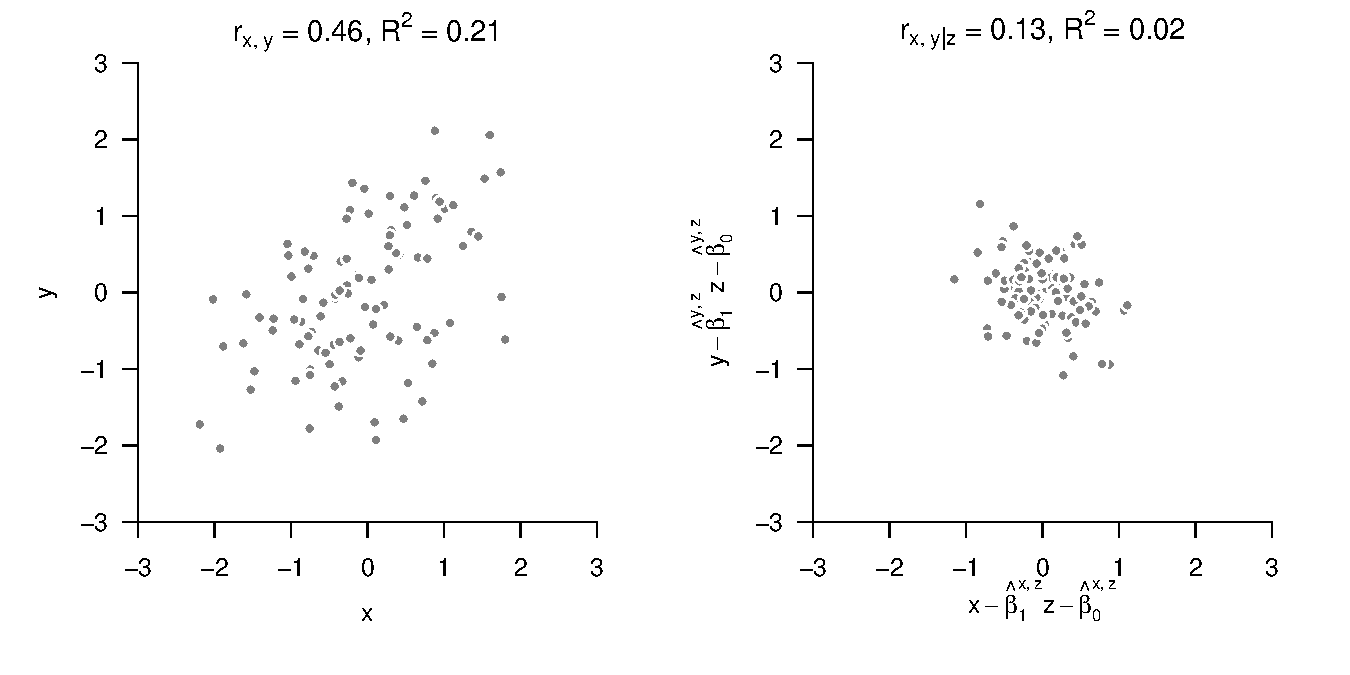
\includegraphics[width=1\linewidth]{2_Abbildungen/alm_2_partielle_korrelation_beispiel} \end{center}
\end{frame}

\begin{frame}{Bedingte Korrelation und Partielle Korrelation}
\protect\hypertarget{bedingte-korrelation-und-partielle-korrelation-14}{}
\vspace{1cm}

\begin{center}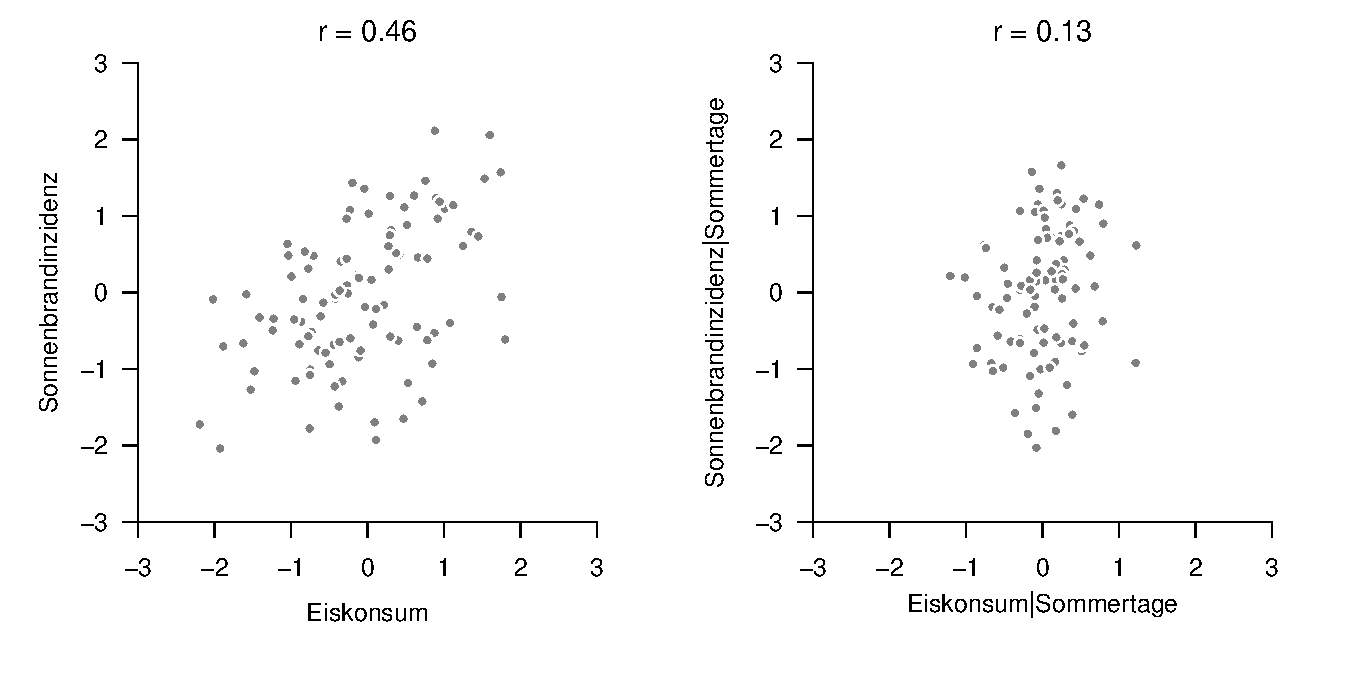
\includegraphics[width=1\linewidth]{2_Abbildungen/alm_2_partielle_korrelation_anwendung} \end{center}
\end{frame}

\begin{frame}{}
\protect\hypertarget{section-8}{}
\setstretch{2}
\vfill
\large

Grundlagen

Korrelation und Bestimmtheitsmaß

Korrelation und lineare Abhängigkeit

Korrelation und Regression

Bedingte Korrelation und Partielle Korrelation

\textbf{Selbstkontrollfragen}

\vfill
\end{frame}

\begin{frame}{Selbstkontrollfragen}
\protect\hypertarget{selbstkontrollfragen}{}
\setstretch{1.8}
\tiny
\justifying

\begin{enumerate}
\tightlist
\item
  Geben Sie die Definition der Korrelation zweier Zufallsvariablen
  wieder.
\item
  Geben Sie die Definitionen von Stichprobenmittel, -standardabweichung,
  -kovarianz und -korrelation wieder.
\item
  Erläutern Sie anhand der Mechanik der Kovariationsterme, wann eine
  Stichprobenkorrelation einen hohen absoluten Wert annimmt, einen hohen
  positiven Wert annimmt, einen hohen negativen Wert annimmt und einen
  niedrigen Wert annimmt.
\item
  Berechnen Sie die Korrelation von Anzahl der Therapiestunden und
  Symptomreduktion anhand der Daten in Beispieldatensatz.csv.
\item
  Geben Sie das Theorem zur Stichprobenkorrelation bei linear-affinen
  Transformationen wieder.
\item
  Erläutern Sie das Theorem zur Stichprobenkorrelation bei
  linear-affinen Transformationen.
\item
  Geben Sie die Definitionen von erklärten Werten und Residuen einer
  Ausgleichsgerade wieder.
\item
  Geben Sie das Theorem zur Quadratsummenzerlegung bei einer
  Ausgleichsgerade wieder.
\item
  Erläutern Sie die intuitiven Bedeutungen von
  \(\mbox{SQT}, \mbox{SQE}\) und \(\mbox{SQR}\).
\item
  Geben Sie die Definition des Bestimmtheitsmaßes \(\mbox{R}^2\) wieder.
\item
  Geben Sie das Theorem zum Zusammenhang von Stichprobenkorrelation und
  Bestimmtheitsmaß wieder.
\item
  Erläutern Sie die Bedeutung von hohen und niedrigen \(\mbox{R}^2\)
  Werten im Lichte der Ausgleichsgerade.
\item
  Berechnen Sie in einem R-Skript \(\mbox{R}^2\) für die Daten in der
  Datei Beispieldatensatz.csv anhand der Definition von \(\mbox{R}^2\).
  Überprüfen Sie Ihr Ergebnis anhand des Theorems zum Zusammenhang von
  Stichprobenkorrelation und Bestimmheitsmaß.
\item
  Geben Sie das Theorem zum Zusammenhang von Korrelation und
  linear-affiner Abhängigkeit wieder.
\item
  Geben Sie die Definition der Regressionsgerade zweier Zufallsvariablen
  wieder.
\item
  Geben Sie das Theorem zur Optimalität der Regressionsgerade zweier
  Zufallsvariablen wieder.
\item
  Geben Sie das Theorem zum Zusammenhang von Korrelation und Regression
  an.
\item
  Erläutern Sie, wie aus den Ergebnissen einer Regressionananlyse das
  Ergebnis einer Korrelationsanalyse errechnet werden kann.
\end{enumerate}
\end{frame}

\begin{frame}{References}
\protect\hypertarget{references}{}
\footnotesize

\hypertarget{refs}{}
\begin{CSLReferences}{1}{0}
\leavevmode\hypertarget{ref-baba_2004}{}%
Baba, Kunihiro, Ritei Shibata, and Masaaki Sibuya. 2004. {``Partial
Correlation and Conditional Correlation as Measures of Conditional
Independence.''} \emph{Australian {\(<\)}Html\_ent Glyph="@amp;"
Ascii="\&amp;"/{\(>\)} New Zealand Journal of Statistics} 46 (4):
657--64. \url{https://doi.org/10.1111/j.1467-842X.2004.00360.x}.

\leavevmode\hypertarget{ref-imbens_2015}{}%
Imbens, Guido, and Donald B. Rubin. 2015. \emph{Causal {Inference} for
{Statistics}, {Social}, and {Biomedical Sciences}: {An Introduction}}.
{Academic Press}.

\leavevmode\hypertarget{ref-lawrance_1976}{}%
Lawrance, A. J. 1976. {``On {Conditional} and {Partial Correlation}.''}
\emph{The American Statistician} 30 (3): 146.
\url{https://doi.org/10.2307/2683864}.

\leavevmode\hypertarget{ref-pearl_2000}{}%
Pearl, Judea. 2000. \emph{Causality: Models, Reasoning, and Inference}.
{Cambridge, U.K. ; New York}: {Cambridge University Press}.

\end{CSLReferences}
\end{frame}

\end{document}
